% =====================================================================
%  Cost Compass
%  디자인적 사고 (SWCON103) 2026학년도 2학기 중간 레포트
%
%  컴파일 : Overleaf 에서 pdfLaTeX
%  참고문헌: BibTeX (refer.bib)  ->  pdfLaTeX, BibTeX, pdfLaTeX x2
%
%  제출용 PDF 를 만들 때만 아래 두 줄을 본인 정보로 바꾼다.
%  공개 저장소에는 자리표시자 상태로 둔다.
% =====================================================================

\documentclass[11pt,a4paper]{article}

\usepackage[hangul]{kotex}
\usepackage[margin=2.4cm]{geometry}
\usepackage{graphicx}
\usepackage{tabularx}
\usepackage{array}
\usepackage{booktabs}
\usepackage{xcolor}
\usepackage{fancyhdr}
\usepackage{enumitem}
\usepackage{caption}
\usepackage[colorlinks=true, linkcolor=blue, citecolor=blue,
            urlcolor=blue]{hyperref}

% ---- 제출자 정보 (제출 시에만 수정) ---------------------------------
\newcommand{\studentid}{(학번)}
\newcommand{\studentname}{(이름)}

% ---- 표/그림 번호를 '장-번호' 형식으로 ------------------------------
\counterwithin{table}{section}
\counterwithin{figure}{section}
\renewcommand{\thetable}{\thesection-\arabic{table}}
\renewcommand{\thefigure}{\thesection-\arabic{figure}}
\captionsetup{labelsep=quad, font=small, labelfont=bf}

% ---- 표 편의 정의 ---------------------------------------------------
\newcolumntype{Y}{>{\raggedright\arraybackslash}X}
\newcolumntype{C}{>{\centering\arraybackslash}X}
\renewcommand{\arraystretch}{1.25}

% 코드 조각: 밑줄을 자동으로 처리한다
\newcommand{\code}[1]{\texttt{\detokenize{#1}}}

% ---- 머리글 ---------------------------------------------------------
\pagestyle{fancy}
\fancyhf{}
\setlength{\headheight}{15pt}
\lhead{디자인적 사고 (SWCON103)}
\chead{\studentname}
\rhead{Cost Compass}
\cfoot{\thepage}

\begin{document}

% =====================================================================
%  표지
% =====================================================================
\begin{titlepage}
\centering
\vspace*{2.5cm}

{\large 디자인적 사고 (SWCON103)}\\[0.4cm]
{\large 2026학년도 2학기 중간 레포트}

\vspace{3.0cm}

{\Huge\bfseries Cost Compass}\\[1.0cm]
{\LARGE 크레딧이 걱정되는 학생을 위한}\\[0.35cm]
{\LARGE 인프라 설계 비용 비교 도구}

\vspace{3.5cm}

{\large 소프트웨어융합학과}\\[0.4cm]
{\large \studentid \quad \studentname}

\vspace{2.0cm}

{\large 담당교수 \quad 조명아}\\[0.3cm]
{\large 제출일 \quad 2026. 11. 4.}

\vspace{1.2cm}

{\small 저장소 \quad \url{https://github.com/philipn337-namphil/cost_compass_maker_movement}}

\vfill
\end{titlepage}

\newpage
\tableofcontents
\thispagestyle{empty}

\newpage
\setcounter{page}{1}

% =====================================================================
\section{서론}

\subsection{메이커가 된다는 것}

메이커 운동은 스스로 필요한 것을 만들고, 만드는 방법을 공유하며 함께 발전시키는 사회적 흐름이다~\cite{anderson2012, dougherty2012}. 수업에서는 메이커가 된다는 것을 세 가지 변화로 정리하였다~\cite{cho2026}.

\begin{table}[!h]
\centering
\caption{메이커가 된다는 것: 세 가지 변화와 본 보고서의 대응}
\label{tab:maker}
\small
\begin{tabularx}{\textwidth}{l Y Y}
\toprule
\textbf{변화} & \textbf{의미} & \textbf{본 보고서에서} \\
\midrule
소비자 $\rightarrow$ \textbf{생산자} & 주어진 제품을 쓰는 데서 그치지 않고 필요한 것을 직접 만든다 & 1.2 $\sim$ 3장 --- 겪은 불편을 `만들 것'으로 바꾸는 과정 \\
아이디어 $\rightarrow$ \textbf{프로토타입} & 머릿속 생각을 작게라도 만들어 보고 확인한다 & 4 $\sim$ 5장 --- 아이디어를 도구로 만들고 실제로 측정 \\
혼자 $\rightarrow$ \textbf{함께} & 만든 방법을 공유하고 다른 사람의 결과물 위에 쌓는다 & 6.2 --- 코드와 측정 결과를 공개 저장소로 \\
\bottomrule
\end{tabularx}
\end{table}

이 가운데 본 프로젝트에서 가장 어려웠던 것은 \textbf{첫 번째 변화}였다. 만드는 일 자체는 오픈소스가 대부분 해결해 주었다. 정작 막힌 것은 ``무엇을 만들 것인가''였다.

강의자료는 이 점을 짚어 다음과 같이 적고 있다.

\begin{quote}
\textbf{왜 지금?} AI가 코드를 대신 써 주는 시대일수록 `무엇을 만들지' 정하는 능력이 중요하다.
\end{quote}

그래서 과제를 받고 처음 한 일은 도구를 고르는 것이 아니라, \textbf{최근 내가 실제로 불편을 겪은 장면을 되짚는 것}이었다. 그 장면에서 출발해 문제를 정의하고, 오픈소스를 엮어 도구를 만들고, 결과를 다시 공개하기까지가 본 보고서의 내용이다.

\subsection{연구 배경: 무엇을 만들지 찾다가}

무엇을 만들지 찾기 위해 최근 몇 달을 돌아보았을 때 가장 먼저 떠오른 것은 클라우드 인프라를 설계하던 경험이었다.

클라우드는 쓴 만큼 돈을 내는 구조이다. 이 구조는 초기 투자 없이 시작할 수 있다는 장점이 있지만, 동시에 \textbf{얼마를 쓰게 될지 미리 알기 어렵다}는 문제를 함께 가져온다.

필자는 AWS로 클라우드 인프라 공부를 시작하였고, 최근 수업과 팀 프로젝트에서 로드 밸런서와 오토 스케일링을 포함한 인프라를 직접 설계해 보았다. 이 과정에서 반복적으로 겪은 불편이 있었다. 여러 구성안을 놓고 어느 것을 택할지 고민할 때, \textbf{성능과 가용성은 비교할 기준이 있었지만 비용은 비교할 방법이 없었다}는 점이다.

성능은 ``인스턴스를 늘리면 처리량이 는다'', 가용성은 ``서버를 두 대로 나누면 한 대가 죽어도 버틴다''처럼 설계 단계에서 따져 볼 수 있다. 그러나 비용은 달랐다. 구성안별로 월 얼마가 나오는지 알려면 결국 리소스를 실제로 만들어 보고 청구서를 기다리는 수밖에 없었다. 그 결과 비용은 설계를 \textbf{고르는 기준}이 되지 못하고, 설계를 \textbf{다 정한 뒤에 통보받는 결과}가 되었다.

특히 학생에게는 이 문제가 훨씬 무겁게 다가온다. 학생은 대개 교육용 크레딧을 받아 실습한다. 크레딧은 한도가 정해져 있고, 한 번 차감되면 되돌릴 수 없으며, 다 써 버리면 남은 학기 동안 실습할 방법 자체가 사라진다. 실무자가 회사 예산으로 실수를 흡수할 수 있는 것과 달리, 학생에게 과금은 \textbf{되돌릴 수 없는 일회성 손실}이다.

그래서 학생은 리소스를 고를 때마다 ``이걸 켜면 크레딧이 얼마나 깎일지 모른다''는 불안을 안고 선택하게 되고, 그 불안은 \textbf{과도하게 보수적인 선택}으로 이어진다. 성능이 더 좋은 인스턴스를 한 번 써 보면 사양에 따라 무엇이 어떻게 달라지는지 체감할 수 있는데도, 얼마가 깎일지 모르니 겁이 나서 가장 작은 사양만 고르게 된다. 로드 밸런서와 오토 스케일링처럼 여러 리소스가 동시에 켜지는 구성은 금액을 가늠할 수 없어 아예 시도조차 못 하는 경우도 있다. 필자 역시 실습 중에 더 큰 인스턴스를 띄워 비교해 보고 싶었으나, 크레딧이 얼마나 줄어들지 알 수 없어 그만둔 적이 있다.

여기서 이 문제의 성격이 분명해진다. 학생이 비용을 몰라서 잃는 것은 \textbf{돈이 아니라 배울 기회}이다. 따라서 학생에게 필요한 것은 ``비용을 아껴 주는 도구''가 아니라, \textbf{얼마가 나올지 미리 알려 주어 안심하고 선택하게 해 주는 도구}이다. 아끼는 것이 목적이라면 아무것도 켜지 않는 것이 최선일 것이나, 그것은 학습을 포기하는 일이다. 문제는 비싸다는 것이 아니라 \textbf{모른다는 것}이다.

\subsection{프로젝트 개요}

본 보고서가 제안하는 것은 \textbf{Cost Compass}이다. 교육용 크레딧으로 실습하는 학생이 \textbf{배포하기 전에} 여러 인프라 설계안의 월 예상 비용을 같은 조건에서 비교하고, 트래픽과 사양 가정을 바꿔 가며 그 차이가 얼마나 벌어지는지 직접 확인할 수 있게 하는 도구이다.

\begin{table}[!h]
\centering
\caption{Cost Compass 개요}
\label{tab:overview}
\small
\begin{tabularx}{\textwidth}{l Y}
\toprule
\textbf{항목} & \textbf{내용} \\
\midrule
사용자 & 교육용 크레딧으로 AWS를 처음 실습하는 학생 \\
해결할 문제 & 비용을 몰라 겁이 나고, 그 결과 가장 작은 사양만 고르게 되어 배울 기회를 잃는 것 \\
제공하는 것 & 설계안 3종의 월 비용 비교, 리소스별 비용 기여도, 트래픽과 사양에 따른 비용 변화 \\
전제 조건 & 클라우드에 \textbf{아무것도 배포하지 않는다.} 크레딧이 차감되지 않는다 \\
공개 저장소 & \code{github.com/philipn337-namphil/cost_compass_maker_movement} \\
\bottomrule
\end{tabularx}
\end{table}

설계안 코드, 설정 파일, 분석 스크립트, 측정 결과, 본 보고서를 모두 공개 저장소에 올려 두었다~\cite{costcompass}. 공개한 이유는 6.2에서 따로 다룬다.

여기서 중요한 점은 이 프로젝트의 중심이 특정 도구가 아니라 \textbf{위의 문제}라는 것이다. 문제를 풀기 위해 다섯 개의 오픈소스를 연결하여 하나의 파이프라인을 구성하였으며, 그 가운데 Infracost가 비용 환산을 담당하는 핵심 부품이다. 각 오픈소스의 역할은 2장에서 다룬다.

\subsection{보고서의 구성}

본 보고서는 1.1에서 제시한 세 가지 변화를 차례로 따라간다.

2장에서는 프로젝트를 구성하는 오픈소스 다섯 가지와 그 연결 구조, 라이선스를 정리한다. 3장에서는 관점 바꾸기와 5 Whys로 근본 원인을 찾고 물리적 모순으로 정의하여 `진짜 문제'를 한 문장으로 도출한다. 여기까지가 \textbf{겪은 불편을 만들 것으로 바꾸는 과정}, 즉 소비자에서 생산자로의 전환에 해당한다.

4장에서는 SCAMPER로 발산 방향을 잡고, 브레인스토밍으로 후보를 나열한 뒤, TRIZ 분리 원리로 모순을 해소하고, 가중 순위 결정법으로 최종안을 선택한다. 5장에서는 그 아이디어를 실제로 만들어 측정한 결과와 한계를 밝힌다. 이 두 장이 \textbf{아이디어에서 프로토타입으로}의 전환이다.

6장에서는 결과를 정리하고, 만든 것을 공개 저장소로 돌려놓은 과정을 다룬다. \textbf{혼자에서 함께로}의 전환이며, 1.1에서 시작한 이야기가 닫히는 지점이다.

% =====================================================================
\section{사용한 오픈소스}

\subsection{전체 파이프라인}

수업에서는 메이커 운동을 이끈 세 가지 힘으로 \textbf{ICT 발전과 오픈소스}, \textbf{3D 프린터}, \textbf{메이커 스페이스}를 들었다. 본 프로젝트는 이 가운데 첫 번째에 전적으로 기대고 있다. 남이 공개한 코드를 가져다 쓸 수 있었기 때문에, 개인이 가격 데이터베이스를 구축하거나 HCL 파서를 직접 작성하지 않고도 도구를 만들 수 있었다.

Cost Compass는 하나의 오픈소스를 쓰는 것이 아니라, 성격이 다른 다섯 개를 \textbf{설계안에서 화면까지 이어지는 한 줄기}로 연결하여 만들어진다.

\begin{figure}[!h]
\centering
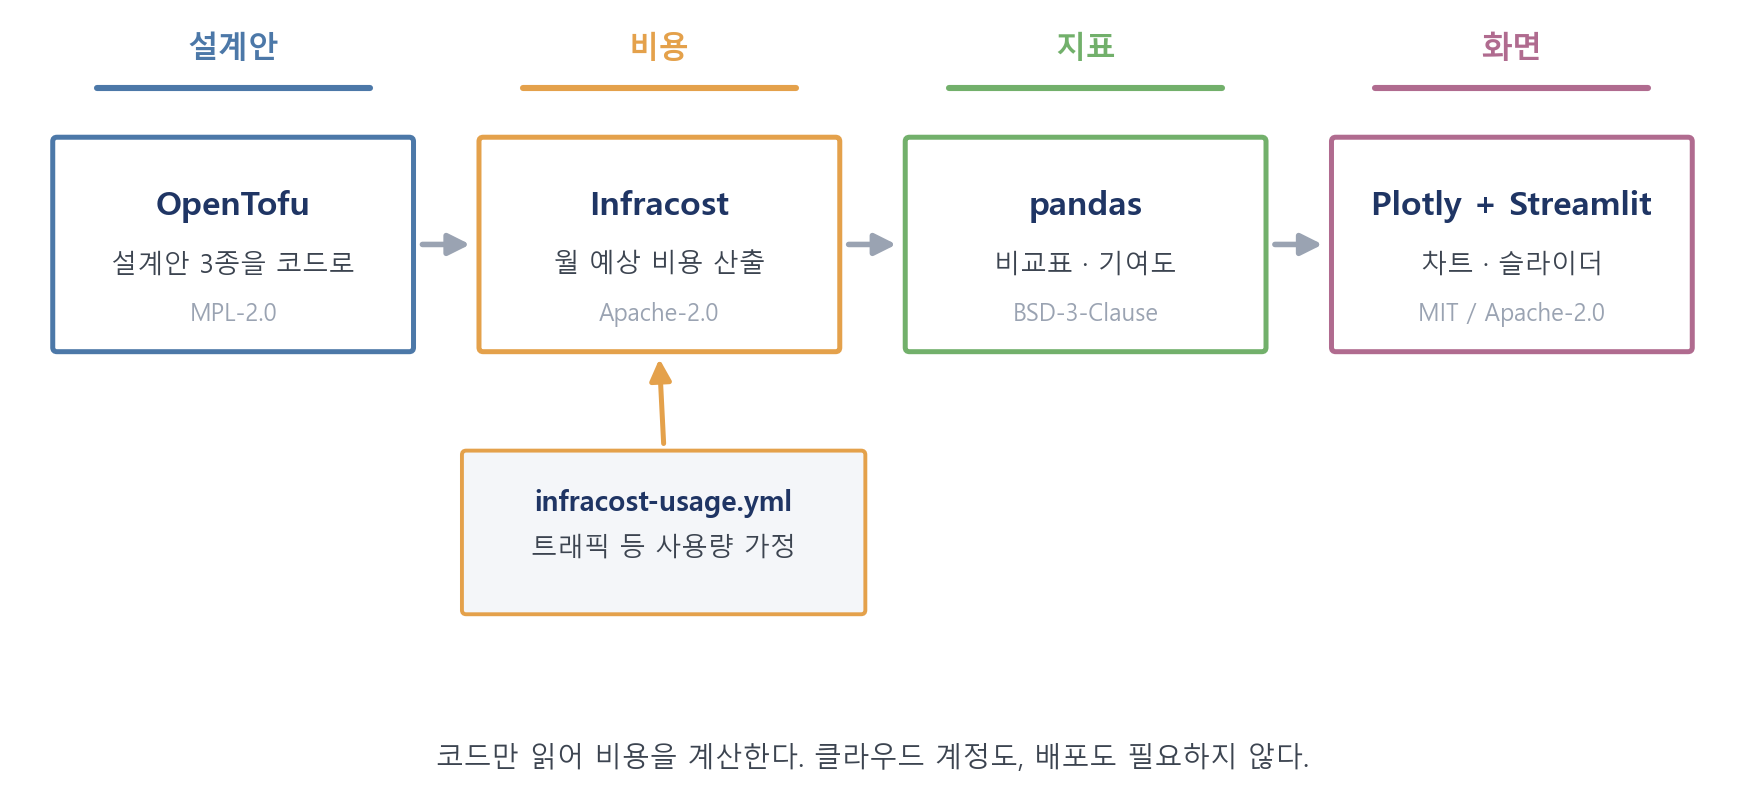
\includegraphics[width=\linewidth]{figure/fig_2_1_pipeline.png}
\caption{Cost Compass의 오픈소스 파이프라인}
\label{fig:pipeline}
\end{figure}

\begin{table}[!h]
\centering
\caption{사용한 오픈소스와 역할}
\label{tab:oss}
\small
\begin{tabularx}{\textwidth}{c l Y l}
\toprule
\textbf{순서} & \textbf{오픈소스} & \textbf{역할} & \textbf{라이선스} \\
\midrule
1 & \textbf{OpenTofu}  & 설계안 3종을 코드로 선언하고 유효성 검증 & MPL-2.0 \\
2 & \textbf{Infracost} & 코드를 읽어 월 예상 비용 산출 & Apache-2.0 \\
3 & \textbf{pandas}    & JSON을 파싱해 설계안별 비용 비교표 생성 & BSD 3-Clause \\
4 & \textbf{Plotly}    & 비용 구성과 비교를 차트로 표현 & MIT \\
5 & \textbf{Streamlit} & 트래픽 슬라이더를 제공해 직접 조작하게 함 & Apache-2.0 \\
\bottomrule
\end{tabularx}
\end{table}

위 라이선스는 2026년 11월 3일, 설치된 패키지의 메타데이터에서 직접 확인하였다(pandas 2.3.2, Plotly 6.9.0, Streamlit 1.66.1)~\cite{pandas, plotly, streamlit}.

이와 별도로, 본 보고서의 그림~\ref{fig:pipeline}과 그림~\ref{fig:flow} 다이어그램을 그리는 데 \textbf{matplotlib}(3.10.8, PSF 계열 라이선스)을 사용하였다. 도구를 구성하는 부품은 아니므로 위 파이프라인에는 포함하지 않았다.

\subsection{Infracost: 설계안을 비용으로 환산한다}

\subsubsection{정의}

Infracost는 \textbf{클라우드 인프라를 실제로 배포하지 않고, 코드만 보고 월 예상 비용을 계산해 주는 오픈소스 도구}이다~\cite{infracostrepo}. Terraform과 같은 코드형 인프라(IaC, Infrastructure as Code) 파일을 입력으로 받아, 그 코드가 배포되었을 때 발생할 비용을 추정하여 출력한다.

\begin{quote}
\textbf{코드형 인프라(IaC)란?}\\
서버 $\cdot$ 네트워크 $\cdot$ 데이터베이스 같은 인프라를 콘솔에서 클릭해서 만드는 대신, 설정을 텍스트 파일로 적어 두고 그 파일을 실행해 만드는 방식이다. 같은 파일을 다시 실행하면 같은 인프라가 다시 만들어지므로, 인프라를 소스 코드처럼 관리할 수 있다.
\end{quote}

\begin{table}[!h]
\centering
\caption{Infracost 기본 정보}
\label{tab:infracost}
\small
\begin{tabularx}{\textwidth}{l Y}
\toprule
\textbf{항목} & \textbf{내용} \\
\midrule
저장소 & \code{github.com/infracost/infracost} \\
라이선스 & Apache License 2.0 \\
지원 입력 & Terraform, Terragrunt, CloudFormation, AWS CDK \\
지원 클라우드 & AWS, Azure, Google Cloud \\
지원 리소스 & 1,100개 이상 \\
제공 형태 & CLI, IDE 확장, CI/CD 풀 리퀘스트 코멘트 \\
GitHub Star & 약 12.6k (2026년 11월 기준) \\
\bottomrule
\end{tabularx}
\end{table}

\subsubsection{동작 원리}

Infracost가 비용을 산출하는 과정은 네 단계로 나눌 수 있다. 전체 흐름은 그림~\ref{fig:flow}와 같다.

\begin{figure}[!h]
\centering
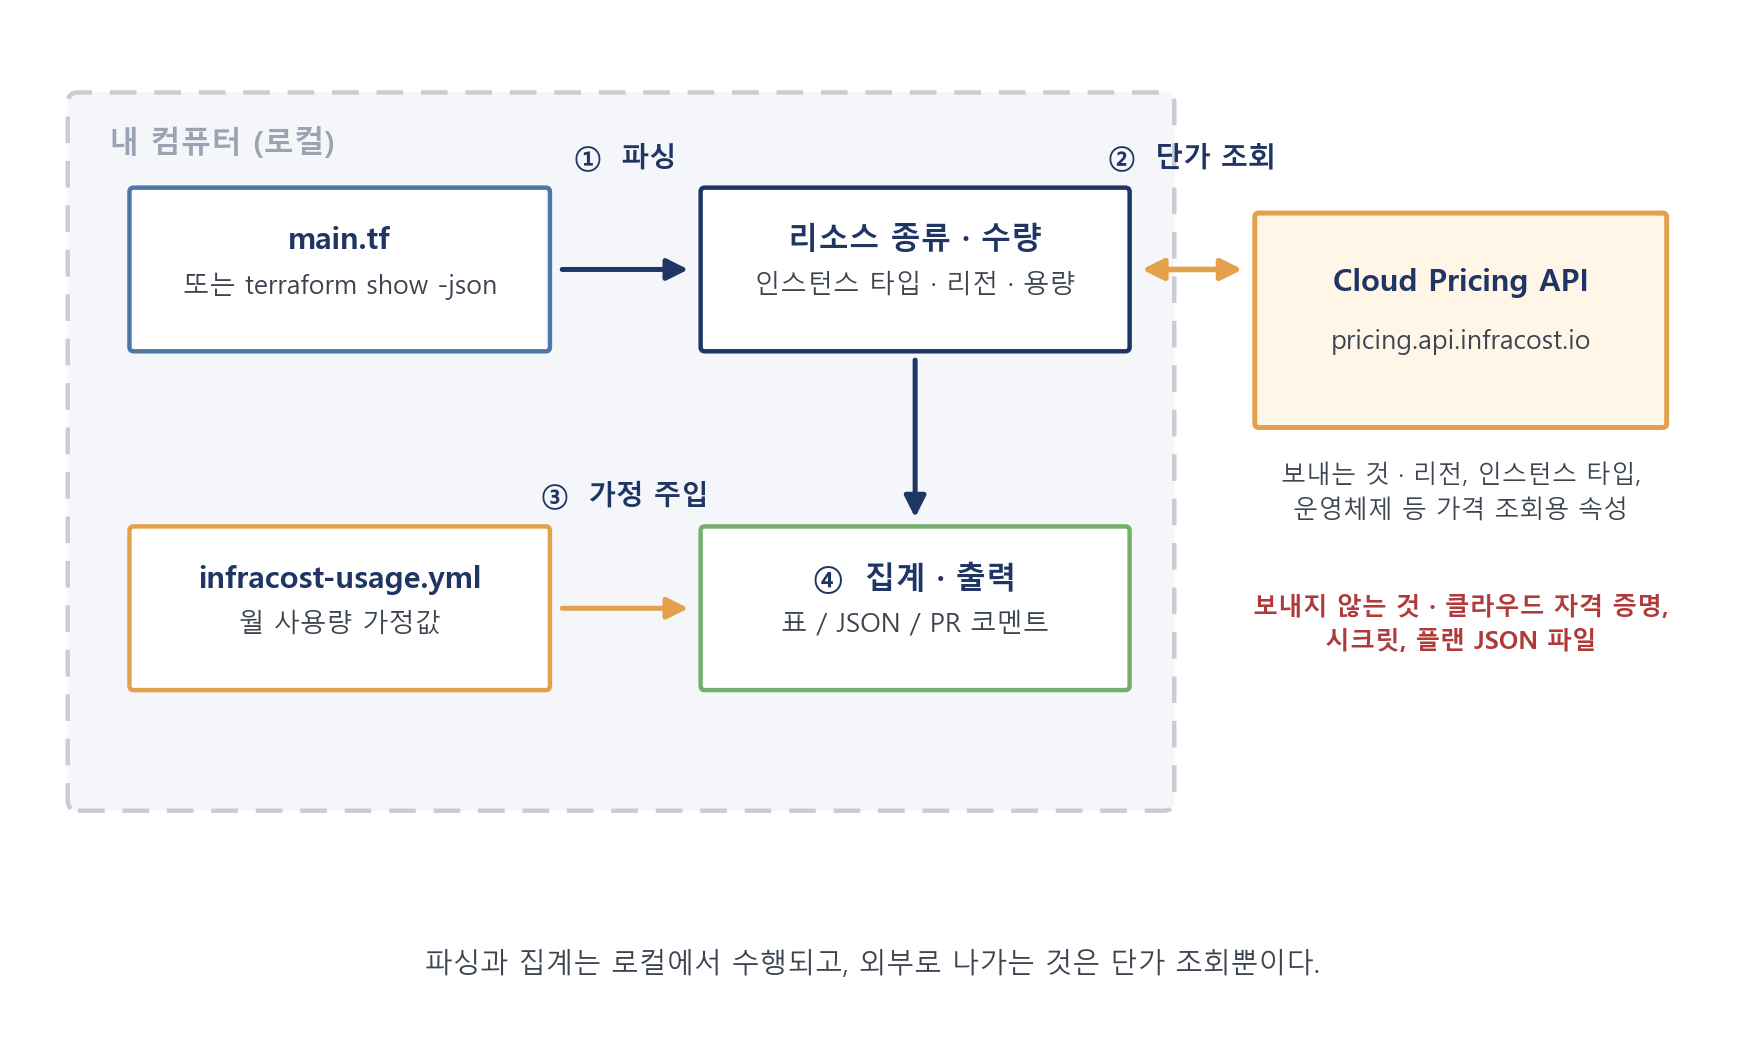
\includegraphics[width=\linewidth]{figure/fig_2_2_infracost_flow.png}
\caption{Infracost의 비용 산출 흐름}
\label{fig:flow}
\end{figure}

\paragraph{(1) 코드 파싱 --- 무엇을 만들 것인지 읽는다 (로컬 수행)}
Infracost는 프로젝트를 \textbf{로컬에서 파싱하여} 생성될 리소스의 종류와 수량을 판단한다. 예를 들어 \code{aws_instance} 리소스에서 인스턴스 타입(\code{t3.small}), 리전, 연결된 스토리지 크기를 읽어 낸다. HCL 파일을 직접 읽을 수도 있고, \code{terraform show -json}으로 생성한 플랜 JSON 파일을 입력으로 받을 수도 있다.

이 단계에서 \textbf{클라우드 계정에 접속하지 않는다.} Infracost는 IaC 상태 파일이나 실제 클라우드 리소스를 변경하지 않으며, 클라우드 자격 증명을 요구하지도 않는다.

이 성질이 Cost Compass의 \textbf{전제 조건 그 자체}이다. 학생이 크레딧 차감 없이 비용을 확인할 수 있는 이유, 그리고 본 보고서가 ``설계 확정 이전''이라는 시점을 다룰 수 있는 이유가 모두 여기에 있다.

\paragraph{(2) 단가 조회 --- Cloud Pricing API에 묻는다}
파싱으로 얻은 속성을 조회 조건으로 삼아, Infracost가 운영하는 \textbf{Cloud Pricing API}(\code{pricing.api.infracost.io})에 단가를 질의한다~\cite{infracostdocs}. 조회 조건에는 공급자, 서비스, 제품군, 리전, 인스턴스 타입, 테넌시, 운영체제, 사전 설치 소프트웨어 등이 포함된다. 같은 인스턴스 타입이라도 리전과 운영체제에 따라 단가가 다르므로, 속성의 \textbf{조합 전체}가 매칭 키가 된다.

이 API를 사용하려면 무료 API 키가 필요하다. 조직 단위로 사용자 지정 가격표나 AWS EDP, Azure EA 같은 할인 계약을 등록해 두면 조회 결과에 반영된다.

\paragraph{(3) 사용량 가정 --- 코드에 없는 값을 채운다}
클라우드 요금은 성격이 다른 \textbf{두 종류}로 나뉜다.

\begin{table}[!h]
\centering
\caption{클라우드 요금의 두 종류}
\label{tab:costtypes}
\small
\begin{tabularx}{\textwidth}{l Y Y c}
\toprule
\textbf{구분} & \textbf{설명} & \textbf{예} & \textbf{코드만으로 알 수 있는가} \\
\midrule
리소스 기반 & 켜 두기만 해도 시간당 부과 & EC2 인스턴스 시간, EBS 용량 & \textbf{알 수 있음} \\
사용량 기반 & 실제로 얼마나 쓰는지에 따라 부과 & 데이터 전송량, S3 요청 수, ALB의 LCU & \textbf{알 수 없음} \\
\bottomrule
\end{tabularx}
\end{table}

사용량 기반 항목은 코드에 적혀 있지 않다. 그래서 Infracost는 \textbf{사용량 파일}(\code{infracost-usage.yml})이라는 별도의 YAML 파일로 이 값을 받는다. 사용량 파일을 주지 않으면 미리 정해진 기본값이 적용되는데, 이는 해당 리소스가 \textbf{공짜가 아니라는 사실을 보이기 위한 장치}이다. 아래는 월 처리 데이터를 100GB로 가정한 예이다.

\begin{quote}
\begin{verbatim}
version: 0.1
resource_type_default_usage:
  aws_lb:
    processed_bytes_gb: 100
resource_usage:
  aws_db_instance.app:
    additional_backup_storage_gb: 0
\end{verbatim}
\end{quote}

이 파일은 \code{infracost.yml}에서 \code{usage_file} 키로 참조한다. 주목할 점은 \textbf{이 구조 자체가 4.3에서 적용할 공간 분리의 근거가 된다}는 것이다. 미리 확정해야 하는 부분(리소스 구성)은 \code{.tf} 파일에, 미리 정할 수 없는 부분(트래픽량)은 \code{infracost-usage.yml}에 나누어 둘 수 있도록 Infracost가 이미 설계되어 있다. Cost Compass의 트래픽 슬라이더는 바로 이 파일의 값을 조작한다.

\paragraph{(4) 집계와 출력}
리소스별 비용을 합산해 월 예상 비용을 산출하고, 터미널 표, JSON, 풀 리퀘스트 코멘트 등으로 내보낸다. Cost Compass는 설계안별 결과를 기계적으로 비교해야 하므로 JSON 출력을 사용하며, 이 JSON이 pandas 단계의 입력이 된다.

\subsection{OpenTofu: 설계안을 코드로 기술한다}

\subsubsection{정의와 역할}

OpenTofu는 인프라를 선언적으로 기술하고 관리하는 코드형 인프라 도구이다~\cite{opentofu}. Cost Compass에서는 \textbf{비교할 설계안 3종을 각각 하나의 코드 묶음으로 표현}하고, 그 설정이 유효한지 검증하는 데 쓰인다.

\begin{table}[!h]
\centering
\caption{OpenTofu 기본 정보}
\label{tab:opentofu}
\small
\begin{tabularx}{\textwidth}{l Y}
\toprule
\textbf{항목} & \textbf{내용} \\
\midrule
저장소 & \code{github.com/opentofu/opentofu} \\
라이선스 & Mozilla Public License v2.0 (MPL-2.0) \\
GitHub Star & 약 30.7k (2026년 11월 기준) \\
거버넌스 & Technical Steering Committee 운영 \\
\bottomrule
\end{tabularx}
\end{table}

\subsubsection{Terraform이 아니라 OpenTofu를 검토한 이유}

IaC 도구로는 Terraform이 가장 널리 쓰이지만, 본 프로젝트에서는 \textbf{라이선스 때문에 OpenTofu를 먼저 검토}하였다.

Terraform은 2023년 8월 라이선스를 BUSL-1.1(Business Source License)로 변경하였다. BUSL은 소스 코드를 공개하지만 일정한 상업적 사용을 제한하므로, \textbf{OSI(Open Source Initiative)가 정의하는 오픈소스에 해당하지 않는다.} OpenTofu는 이 변경에 대응해 만들어진 포크로, MPL-2.0을 유지한다.

``오픈소스를 활용하라''는 본 과제의 취지에 비추어 보면, 파이프라인의 출발점에 놓이는 도구가 엄밀한 의미의 오픈소스인지 여부는 그냥 넘길 문제가 아니다. 이에 따라 OpenTofu를 선택하였다.

\subsubsection{OpenTofu로 설계안을 검증하다}

작성한 설계안이 문법만 그럴듯하고 실제로는 성립하지 않는 설정일 수 있으므로, OpenTofu 1.13.1로 세 설계안을 모두 검사하였다.

\begin{table}[!h]
\centering
\caption{OpenTofu 검증 결과}
\label{tab:tofuvalidate}
\small
\begin{tabularx}{\textwidth}{l Y c c c}
\toprule
\textbf{명령} & \textbf{확인하는 것} & \textbf{A안} & \textbf{B안} & \textbf{C안} \\
\midrule
\code{tofu fmt -check} & HCL 문법과 표준 서식 & 통과 & 통과 & 통과 \\
\code{tofu init}       & 필요한 프로바이더 해석 & 통과 & 통과 & 통과 \\
\code{tofu validate}   & 설정의 유효성(속성, 참조, 타입) & 통과 & 통과 & 통과 \\
\bottomrule
\end{tabularx}
\end{table}

\subsubsection{예상하지 못했던 점: Infracost는 OpenTofu 없이도 동작한다}

검증 과정에서 알게 된 사실이 있다. \textbf{본 프로젝트의 비용 측정은 OpenTofu를 설치하기 전에 이미 모두 끝나 있었다.} Terraform도 OpenTofu도 설치되지 않은 상태에서 Infracost가 \code{.tf} 파일을 읽어 비용을 산출한 것이다.

Infracost가 \textbf{자체 HCL 파서를 내장}하고 있기 때문이다. 2.2.2에서 ``코드를 로컬에서 파싱한다''고 서술한 것이 이 의미이며, 파싱을 위해 IaC 도구를 따로 설치할 필요가 없다.

이 성질은 본 프로젝트의 사용자에게 특히 유리하다. 비용을 비교해 보려는 학생이 설치해야 하는 것은 Infracost 하나뿐이고, IaC 도구 설치와 프로바이더 내려받기(수백 MB)를 건너뛸 수 있다. 1.2에서 밝힌 진입 장벽 관점에서 의미 있는 차이다.

따라서 두 도구의 역할은 서로 다르며 대체 관계가 아니다.

\begin{center}
\small
\begin{tabularx}{0.95\textwidth}{l Y Y}
\toprule
\textbf{도구} & \textbf{역할} & \textbf{없으면} \\
\midrule
OpenTofu  & 설계안이 \textbf{유효한 설정인지 검증} & 잘못된 설정을 모른 채 비용만 계산하게 된다 \\
Infracost & 설계안의 \textbf{비용을 산출}         & 비교 자체가 불가능하다 \\
\bottomrule
\end{tabularx}
\end{center}

\subsection{pandas, Plotly, Streamlit: 비교하고 보여 준다}

Infracost가 내놓는 것은 설계안 \textbf{하나}에 대한 JSON이다. 이를 여러 설계안에 걸쳐 비교 가능한 형태로 바꾸고 학생이 조작할 수 있게 만드는 것이 나머지 세 도구의 역할이다.

\begin{table}[!h]
\centering
\caption{후속 처리 도구의 역할}
\label{tab:posttools}
\small
\begin{tabularx}{\textwidth}{l Y Y}
\toprule
\textbf{오픈소스} & \textbf{원래 용도} & \textbf{Cost Compass에서의 역할} \\
\midrule
\textbf{pandas} & 표 형태 데이터의 가공과 분석 & 설계안 3종의 JSON을 하나의 표로 합치고, 리소스별 비용 기여도와 A안 대비 증감을 계산 \\
\textbf{Plotly} & 대화형 데이터 시각화 & 설계안별 비용 구성을 누적 막대그래프로, 가정에 따른 비용 변화를 그래프로 표현 \\
\textbf{Streamlit} & 파이썬 스크립트를 웹 앱으로 전환 & 트래픽 슬라이더를 제공하여, 학생이 가정을 바꿔 가며 비용 변화를 직접 확인하게 함 \\
\bottomrule
\end{tabularx}
\end{table}

\textbf{Streamlit을 쓰는 이유는 단순히 화면이 필요해서가 아니다.} 1.2에서 규정했듯 이 프로젝트가 다루는 것은 \textbf{불안}이다. 불안은 고정된 표 하나로는 풀리지 않는다. ``트래픽이 이보다 늘면 어떻게 되지?''라는 의문이 남는 한 학생은 여전히 확신 없이 선택하게 된다. 슬라이더를 직접 움직여 가정에 따라 금액이 어떻게 움직이는지 눈으로 확인할 때, 비로소 비용은 불안의 원인이 아니라 판단의 근거가 된다.

\subsection{데이터 처리 경계}

오픈소스를 사용할 때에는 내 데이터가 어디까지 외부로 나가는지 확인해야 한다. Cost Compass의 다섯 도구 가운데 외부와 통신하는 것은 \textbf{Infracost뿐}이며, 나머지는 모두 로컬에서 동작한다.

\begin{table}[!h]
\centering
\caption{외부로 전송되는 것과 전송되지 않는 것 (Infracost 기준)}
\label{tab:boundary}
\small
\begin{tabularx}{\textwidth}{l Y}
\toprule
\textbf{구분} & \textbf{항목} \\
\midrule
\textbf{전송되지 않음} & 클라우드 자격 증명 및 시크릿 \\
                      & Terraform 플랜 JSON 파일 \\
\midrule
\textbf{전송됨} & 가격 조회용 속성 (리전, 인스턴스 타입, 운영체제, 테넌시 등) \\
                & Terraform 리소스 타입별 개수 \\
                & 오류 추적 이벤트 (운영체제, Terraform 버전, CI 종류, Infracost 버전) \\
\bottomrule
\end{tabularx}
\end{table}

정리하면 \textbf{``무엇을 만들 것인가''의 구조적 특징은 나가지만, ``누구의 계정인가''와 코드 전문은 나가지 않는다.} 본 프로젝트는 학습용으로 작성한 설계안만 다루므로 민감 정보가 없다. 다만 실무 환경이라면 리소스 구성 자체가 내부 정보일 수 있으므로, 이 경계를 확인하고 사용할 필요가 있다.

\subsection{라이선스 종합과 선정 판단}

\begin{table}[!h]
\centering
\caption{사용한 오픈소스의 라이선스}
\label{tab:licenses}
\small
\begin{tabularx}{\textwidth}{l l Y Y}
\toprule
\textbf{오픈소스} & \textbf{라이선스} & \textbf{성격} & \textbf{본 프로젝트 사용에 제약} \\
\midrule
OpenTofu  & MPL-2.0       & 파일 단위 약한 카피레프트 & 없음 (수정 없이 사용) \\
Infracost & Apache-2.0    & 허용적, 특허 조항 포함   & 없음 \\
pandas    & BSD 3-Clause  & 허용적                  & 없음 \\
Plotly    & MIT           & 허용적                  & 없음 \\
Streamlit & Apache-2.0    & 허용적                  & 없음 \\
\bottomrule
\end{tabularx}
\end{table}

다섯 도구 모두 수정 없이 호출하여 사용하였으므로, 출처와 라이선스를 참고문헌에 표기하는 것으로 의무를 충족한다. 수업 과제 제출 및 공개 저장소 게시에 제약이 없다.

다만 라이선스만 보고 판단해서는 안 되는 지점이 두 가지 있었다.

\textbf{첫째, Terraform의 사례이다.} 2.3에서 보았듯 가장 널리 쓰이는 도구가 반드시 오픈소스인 것은 아니다. 관행적으로 ``오픈소스''라 불리는 도구라도 라이선스를 직접 확인해야 한다는 점을 이 과정에서 확인하였다.

\textbf{둘째, Infracost의 구조이다.} CLI는 Apache-2.0이지만 가격 데이터는 Infracost가 운영하는 호스팅 API에 의존한다. 즉 \textbf{라이선스가 허용하는 자유와 실제로 독립적으로 운용할 수 있는 범위가 일치하지 않는다.} 오프라인 환경에서 쓰거나 가격 데이터까지 직접 통제해야 하는 상황이라면 이 의존성이 제약이 된다. 본 프로젝트는 인터넷이 연결된 학습 환경에서 설계안을 비교하는 용도이므로 이 제약이 문제가 되지 않는다고 판단하여 Infracost를 선택하였다.

% =====================================================================
\section{문제 창안}

\subsection{관점 바꾸기: 사용자를 바꾸면 전제가 달라진다}

Infracost가 상정하는 기본 사용 맥락은 다음과 같다.

\begin{quote}
이미 Terraform으로 인프라를 관리하고 있고, CI/CD 파이프라인이 갖춰진 팀에서, 엔지니어가 풀 리퀘스트를 올리면 ``이 변경이 월 비용을 얼마나 바꾸는가''가 자동으로 코멘트로 달린다.
\end{quote}

여기서 사용자를 \textbf{교육용 크레딧으로 실습하는 학생}으로 바꾸어 보면, 위 맥락의 전제가 하나씩 무너진다.

\begin{table}[!h]
\centering
\caption{사용자 전환에 따른 전제의 변화}
\label{tab:premise}
\small
\begin{tabularx}{\textwidth}{l Y Y}
\toprule
\textbf{전제} & \textbf{실무 엔지니어} & \textbf{인프라를 처음 설계하는 학생} \\
\midrule
IaC 코드      & 이미 있다 & 아직 없다 \\
비교 대상     & 변경 전 / 변경 후 & 아직 정하지 않은 여러 안 \\
필요한 답     & 얼마나 늘어나는가 & 어느 것을 고를 것인가 \\
재원          & 회사 예산, 추가 집행 가능 & 교육용 크레딧, 한도가 정해져 있음 \\
과금이 생기면 & 비용으로 처리하고 넘어감 & 되돌릴 수 없이 차감, 남은 학기 실습이 막힘 \\
모를 때의 행동 & 일단 배포하고 확인 & \textbf{겁이 나서 가장 작은 사양만 선택} \\
잃는 것       & 돈 & \textbf{배울 기회} \\
비용의 역할   & 통제 기준 & \textbf{선택 기준} \\
\bottomrule
\end{tabularx}
\end{table}

이 표에서 보이듯, 사용자를 바꾸면 Infracost가 답해 주던 질문(``얼마나 늘어나는가'')과 새 사용자가 던지는 질문(``어느 것을 고를 것인가'')이 서로 다르다. 이 간극이 본 보고서의 출발점이다.

\subsection{5 Whys로 근본 원인 찾기}

\textbf{문제 현상:} 학생이 인프라 설계안을 고를 때 비용을 근거로 쓰지 못하고, 얼마가 차감될지 몰라 가장 작은 사양만 선택하게 된다.

\begin{table}[!h]
\centering
\caption{5 Whys 전개}
\label{tab:fivewhys}
\small
\begin{tabularx}{\textwidth}{l Y Y}
\toprule
 & \textbf{질문} & \textbf{답} \\
\midrule
Why 1 & 왜 비용을 근거로 쓰지 못했는가? & 설계 시점에 각 안이 월 얼마인지 알 수 없었기 때문이다. \\
Why 2 & 왜 알 수 없었는가? & 비용을 확인하려면 리소스를 실제로 만들어 보고 청구서를 기다려야 했기 때문이다. \\
Why 3 & 왜 만들어 봐야만 했는가? & 콘솔의 요금 안내는 리소스 하나하나의 단가만 보여 줄 뿐, 구성 전체의 합계를 보여 주지 않았기 때문이다. \\
Why 4 & 왜 구성 단위로는 보이지 않았는가? & 가격표는 리소스 단위로 정의되어 있는데, 설계안은 여러 리소스의 \textbf{조합}이기 때문이다. \\
Why 5 & 왜 조합 단위 비용을 미리 구할 수 없었는가? & 조합을 비용으로 환산하려면 인스턴스 타입, 개수, 리전까지 모두 확정해야 하는데, \textbf{무엇으로 확정할지를 정하려고 비용을 보려던 것}이었기 때문이다. \\
\bottomrule
\end{tabularx}
\end{table}

\textbf{근본 원인:} 비용을 알려면 설계를 확정해야 하고, 설계를 확정하려면 비용을 알아야 하는 \textbf{순환 구조}가 존재한다.

\subsection{물리적 모순 정의}

5 Whys의 마지막 답에서 드러난 순환 구조를, 하나의 특성이 동시에 반대되는 두 값을 가져야 하는 \textbf{물리적 모순}으로 정의한다.

\begin{table}[!h]
\centering
\caption{물리적 모순표}
\label{tab:contradiction}
\small
\begin{tabularx}{\textwidth}{l Y Y}
\toprule
\textbf{특성: 설계안의 구체성} & \textbf{(a) 구체적이어야 한다} & \textbf{($-$a) 구체적이지 않아야 한다} \\
\midrule
\textbf{필수조건(목적)} & 비용을 계산하려면 인스턴스 타입, 개수, 리전, 스토리지 종류가 모두 정해져 있어야 한다. & 여러 안을 비교하는 단계이므로 아직 하나로 확정하지 않은 상태여야 한다. \\
\textbf{어긋나는 점} & 모든 안을 끝까지 구체화하면, 비교를 시작하기도 전에 설계를 여러 벌 완성해야 한다. & 구체화하지 않으면 비용을 전혀 계산할 수 없어 비교 자체가 불가능하다. \\
\bottomrule
\end{tabularx}
\end{table}

\textbf{기술적 모순:} 비교하는 설계안의 수를 늘리면 선택의 폭은 넓어지지만(개선), 각 안을 코드로 구체화하는 데 드는 시간이 선형으로 증가한다(악화).

\subsection{진짜 문제 정의}

\begin{quote}
\textcolor{blue}{\textbf{``교육용 크레딧으로 실습하는 학생이 설계를 확정하지 않은 상태에서도 여러 구성안의 비용을 비교하고 안심하고 선택할 수 있도록, 설계안을 같은 가정 아래 비용으로 환산해 나란히 보여 주는 도구를 만들자.''}}
\end{quote}

% =====================================================================
\section{아이디어 도출}

\subsection{SCAMPER: 발산 방향 설정}

아이디어를 내기 전에, SCAMPER로 \textbf{어느 방향으로 생각을 밀어 볼지}를 먼저 정리하였다.

\begin{table}[!h]
\centering
\caption{SCAMPER 적용}
\label{tab:scamper}
\small
\begin{tabularx}{\textwidth}{l Y Y}
\toprule
\textbf{항목} & \textbf{질문} & \textbf{도출된 방향} \\
\midrule
\textbf{S} 대체     & 무엇을 무엇으로 바꿀까? & 배포 후 청구서를 배포 전 코드로 \\
\textbf{C} 결합     & 무엇과 합칠까? & 비용을 가용성, 성능과 한 화면에 \\
\textbf{A} 응용     & 다른 데서 뭘 빌려올까? & 코드 리뷰의 diff 개념을 설계안 비교에 \\
\textbf{M} 변형     & 크기나 형태를 바꾸면? & 총액 하나를 리소스별 기여도 비율로 분해 \\
\textbf{P} 용도 변경 & 다른 용도로 쓰면? & CI 통과 기준을 설계 학습과 의사결정 보조로 \\
\textbf{E} 제거     & 무엇을 없앨까? & 사용자가 직접 IaC 코드를 작성하는 단계를 없앤다 \\
\textbf{R} 역발상   & 거꾸로 하면? & 설계에서 비용을 구하는 대신, \textbf{예산에서 가능한 설계를 구한다} \\
\bottomrule
\end{tabularx}
\end{table}

\subsection{브레인스토밍: 후보 나열}

SCAMPER가 제시한 방향을 따라 구체적인 아이디어를 발산하였다. 이 단계에서는 실현 가능성을 따지지 않고 양을 우선하였다.

\begin{enumerate}[itemsep=1pt, topsep=4pt]
\item 대표 설계안 3종을 코드 템플릿으로 미리 만들어 두고 한 번에 비용 비교
\item 트래픽 가정값을 바꿔 가며 비용 곡선을 그려 설계안 간 손익분기점 찾기
\item 설계안별로 비용 기여도 상위 3개 리소스를 자동 표시
\item A안을 기준으로 B안과 C안의 증감을 diff 형태로 표시
\item 월 예산을 입력하면 초과하는 설계안과 초과 항목을 경고
\item 비용과 가용성을 두 축으로 하는 산점도에 설계안을 배치
\item 입문자가 자주 놓치는 과금 항목(NAT Gateway, 미사용 EBS 볼륨, 고정 IP 등) 체크리스트 자동 생성
\item 비교 결과를 표로 내보내 설계 문서에 바로 붙이기
\item 같은 설계안을 리전만 바꿔 비교
\item 예산을 입력하면 그 안에서 가능한 구성을 역으로 제시
\end{enumerate}

\subsection{TRIZ 분리 원리: 모순 해소}

브레인스토밍 결과를 그대로 고르지 않고, 3.3에서 정의한 물리적 모순을 \textbf{실제로 해소하는가}를 기준으로 네 가지 분리 원리를 적용하였다.

\begin{table}[!h]
\centering
\caption{분리 원리별 분리질문과 일반해결책}
\label{tab:separation}
\small
\begin{tabularx}{\textwidth}{l Y Y}
\toprule
\textbf{분리원리} & \textbf{분리질문} & \textbf{일반해결책} \\
\midrule
\textbf{시간 분리} & 설계안이 항상 구체적이어야 할까? 아니면 특정 시점에만 구체적이면 될까? & 구체화 작업을 \textbf{비교 시점보다 앞으로} 옮긴다. 대표 설계안을 미리 코드로 만들어 두면, 사용자는 비교 시점에 고르기만 하면 된다. \\
\textbf{공간 분리} & 설계안의 모든 부분이 구체적이어야 할까? 아니면 일부만 구체적이면 될까? & 구체적이어야 하는 부분(인스턴스 타입, 리전, 리소스 구성)과 추상적이어도 되는 부분(트래픽량, 요청 수)을 \textbf{나눈다.} 전자는 템플릿에 고정하고, 후자는 변수로 남긴다. \\
\textbf{조건 분리} & 모든 상황에서 정확해야 할까? 아니면 특정 상황에서만 정확하면 될까? & 비교 단계에서는 \textbf{상대적 순서}만 맞으면 되고, 확정 단계에서만 절대값의 정확도를 높인다. \\
\textbf{전체와 부분 분리} & 전체가 하나의 숫자여야 할까? & 전체는 설계안 단위 총액으로 비교하되, 부분은 리소스 단위로 분해하여 어디서 차이가 나는지 보여 준다. \\
\bottomrule
\end{tabularx}
\end{table}

\textbf{채택: 시간 분리 + 공간 분리}

시간 분리는 ``구체화해야 비교할 수 있는데, 비교해야 구체화할 대상을 정한다''는 순환을 끊는다. 구체화를 \textbf{미리} 해 두면, 사용자 입장에서 비교 시점의 구체성은 0이면서도 계산에 필요한 구체성은 100이 된다. 공간 분리는 여기에 더해, 미리 정할 수 없는 트래픽을 변수로 빼내어 템플릿 하나로 여러 시나리오를 다룰 수 있게 한다.

이 두 가지를 합치면 모순표의 (a)와 ($-$a)가 동시에 성립한다. \textbf{계산기 입장에서 설계안은 완전히 구체적이고(a), 사용자 입장에서 설계안은 아직 확정되지 않았다($-$a).}

덧붙이면, 공간 분리는 Infracost의 구조 위에서 그대로 구현된다. 2.2.2에서 보았듯 Infracost는 리소스 구성을 \code{.tf} 파일로, 사용량 가정을 \code{infracost-usage.yml} 파일로 \textbf{이미 분리해 두고 있다.} 분리 원리로 도출한 해결책이 도구의 기존 구조와 맞아떨어진다는 점은, 이 방향이 무리한 변형이 아님을 뒷받침한다.

\subsection{가중 순위 결정법: 최종 선택}

분리 원리를 통과한 후보 세 가지를 가중 순위 결정법으로 비교하였다.

\begin{itemize}[itemsep=1pt, topsep=4pt]
\item \textbf{후보 1} 설계안 비용 비교 시트 (브레인스토밍 1, 3, 4, 8)
\item \textbf{후보 2} 트래픽 변화에 따른 손익분기 그래프 (브레인스토밍 2, 6)
\item \textbf{후보 3} 예산 역산 설계 추천기 (브레인스토밍 10)
\end{itemize}

평가 기준에는 서로 다른 무게를 주었다. 본 과제의 핵심이 모순 해소에 있으므로 그 항목에 가장 높은 가중치 5를 두었고, 기간 안에 만들어 확인할 수 있는지를 그다음으로 보았다. 각 항목은 1점에서 5점으로 평가하고, \textbf{점수 $\times$ 가중치}의 합으로 순위를 정하였다.

\begin{table}[!h]
\centering
\caption{가중 순위 결정법}
\label{tab:weighted}
\small
\begin{tabularx}{\textwidth}{Y c c c c}
\toprule
\textbf{평가 기준} & \textbf{가중치} & \textbf{후보 1} & \textbf{후보 2} & \textbf{후보 3} \\
\midrule
3.3의 모순을 직접 해소하는가        & 5 & 5 & 3 & 2 \\
보고서 기간 내 구현 가능한가        & 4 & 5 & 3 & 1 \\
학생의 불안을 실제로 줄이는가       & 4 & 4 & 5 & 5 \\
Infracost를 원래 용도와 다르게 쓰는가 & 3 & 4 & 4 & 5 \\
결과를 보고서 안에서 검증할 수 있는가 & 2 & 5 & 2 & 1 \\
\midrule
\textbf{가중 합계} & & \textbf{83} & \textbf{63} & \textbf{51} \\
\bottomrule
\end{tabularx}
\end{table}

\begin{table}[!h]
\centering
\caption{점수를 매긴 근거}
\label{tab:weightedreason}
\footnotesize
\begin{tabularx}{\textwidth}{l Y Y Y}
\toprule
\textbf{기준} & \textbf{후보 1 비교 시트} & \textbf{후보 2 손익분기 그래프} & \textbf{후보 3 예산 역산} \\
\midrule
모순 해소 & \textbf{5} 대표 설계안을 미리 코드로 준비하는 구조 자체가 시간 분리이고, 사용량만 변수로 빼는 것이 공간 분리다 & \textbf{3} 비교는 되지만 이미 구체화된 안들을 전제하므로 `구체성' 모순을 직접 건드리지 않는다 & \textbf{2} 비용에서 설계를 역산하므로 방향이 반대이고, 모순을 우회할 뿐 해소하지 않는다 \\
구현 가능 & \textbf{5} Infracost의 JSON 출력과 pandas만으로 완결된다 & \textbf{3} 트래픽 구간마다 반복 실행과 자동화가 필요해 공수가 늘어난다 & \textbf{1} 가능한 구성의 탐색 공간을 먼저 정의해야 하며, 보고서 기간 안에는 불가능하다 \\
불안 감소 & \textbf{4} 금액을 알게 되지만 정해진 가정 한 벌에 대한 답이다 & \textbf{5} ``어디까지 괜찮은가''를 보여 주므로 불안 해소에 가장 직접적이다 & \textbf{5} 예산 안에서만 고르게 하므로 초과 걱정이 사라진다 \\
용도 전환 & \textbf{4} 단일 코드베이스의 비용에서 설계안 사이의 비교로 단위를 바꾼다 & \textbf{4} 한 시점의 금액에서 구간별 변화로 바꾼다 & \textbf{5} 설계에서 비용을 구하는 방향을 비용에서 설계로 뒤집는다 \\
검증 가능 & \textbf{5} 세 설계안을 한 번 측정하면 표와 그림이 바로 나온다 & \textbf{2} 여러 구간을 측정해야 하고, 교차점이 실제로 존재할지 미리 보장할 수 없다 & \textbf{1} 추천 결과가 타당한지 판단할 기준을 따로 세워야 한다 \\
\bottomrule
\end{tabularx}
\end{table}

\textbf{최종 선택: 후보 1 (83점)}

다만 후보 2가 `불안 감소' 항목에서 유일하게 5점을 받았다는 점은 그대로 버리기 아까웠다. 이 프로젝트가 줄이려는 것이 바로 불안이기 때문이다. 그래서 \textbf{후보 1을 본체로 삼되, 후보 2를 트래픽 슬라이더 형태로 흡수}하였다. 곡선을 따로 그리는 대신 사용자가 가정을 직접 움직여 변화를 확인하게 하면, 구현 공수를 크게 늘리지 않으면서 후보 2의 장점을 가져올 수 있다고 보았다.

후보 3은 전환의 폭이 가장 크지만(용도 전환 5점) 기간 안에 만들 수 없어 제외하고, 6.3의 향후 계획으로 남겼다.

\subsection{최종 아이디어: Cost Compass}

\begin{figure}[!h]
\centering
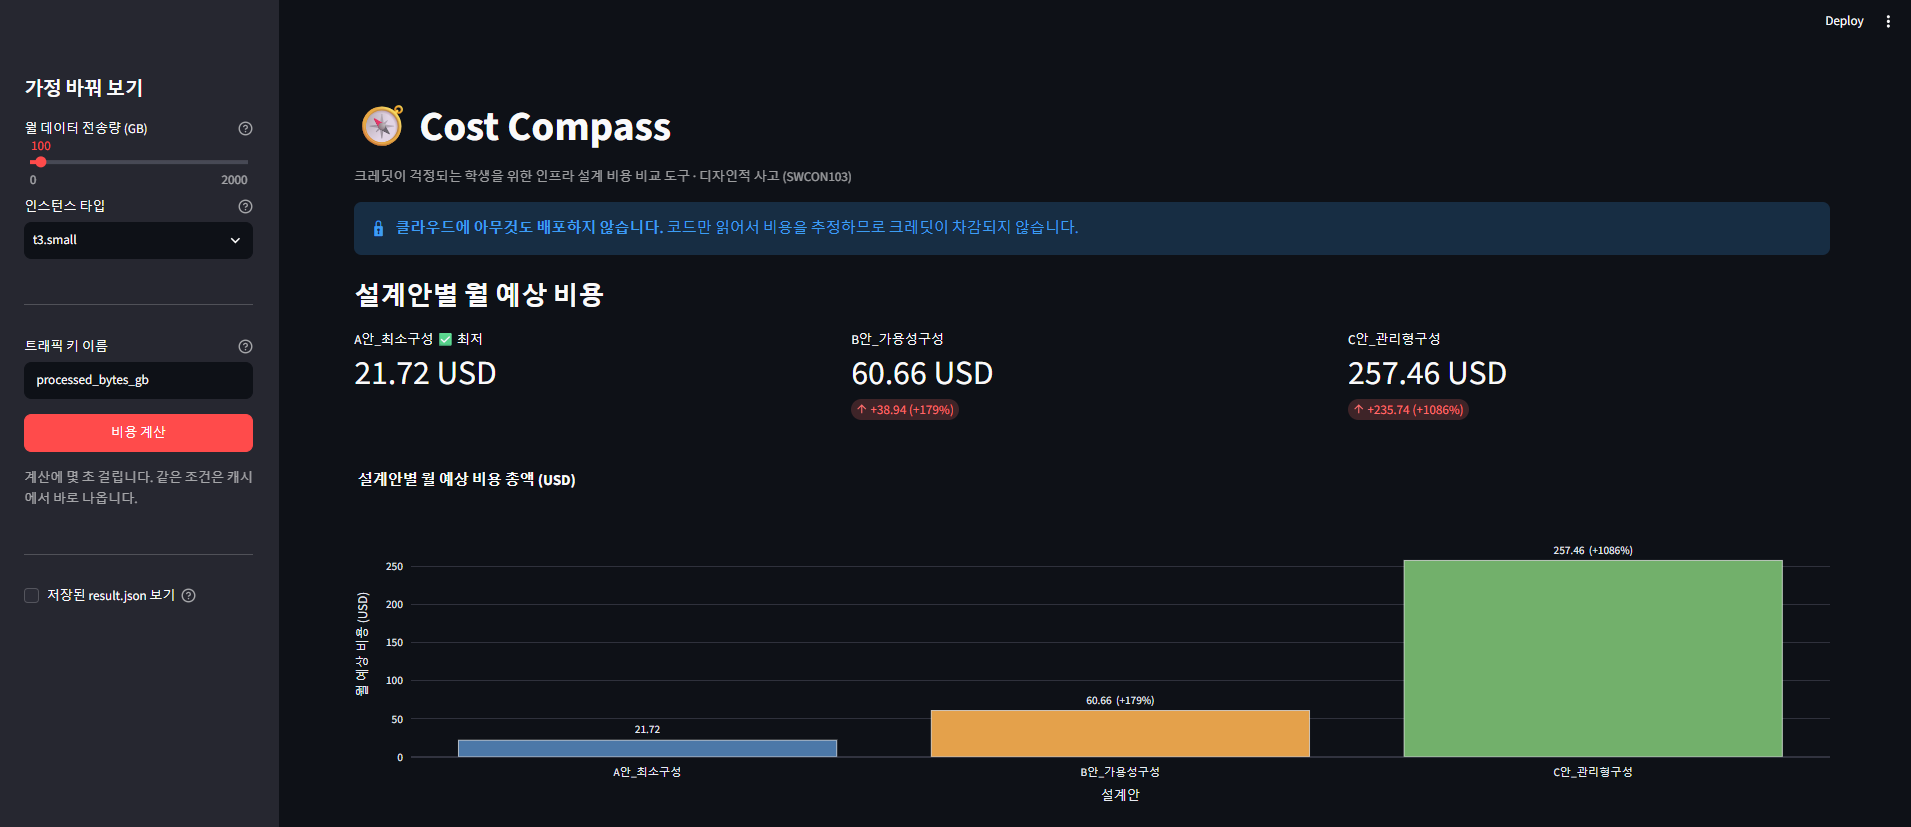
\includegraphics[width=\linewidth]{figure/fig_4_1_screen.png}
\caption{Cost Compass 화면 구성}
\label{fig:screen}
\end{figure}

왼쪽 사이드바에서 월 데이터 전송량과 인스턴스 타입을 바꾸면, 오른쪽의 설계안별 비용과 증감률이 즉시 다시 계산된다. 설계안 코드(\code{.tf})는 그대로 둔 채 사용량 가정만 조작한다는 점에서, 4.3에서 채택한 \textbf{공간 분리가 화면에 그대로 구현되어 있다.}

\textbf{구성}

\begin{itemize}[itemsep=1pt, topsep=4pt]
\item 대표적인 웹 서비스 인프라 설계안 3종을 OpenTofu 템플릿으로 미리 준비한다. \textit{(시간 분리)}
\item 트래픽량 등 사용량 기반 항목은 사용량 파일로 분리하여 변수로 둔다. \textit{(공간 분리)}
\item Infracost를 JSON 출력 모드로 실행하여 설계안별 비용을 수집하고, pandas로 하나의 비교표로 합친다.
\item 설계안별 월 비용 비교표, 리소스별 기여도, A안 대비 증감을 Plotly 차트로 함께 보여 준다. \textit{(전체와 부분 분리)}
\item Streamlit 슬라이더로 트래픽 가정을 바꾸면 비용과 증감률이 즉시 갱신된다. \textit{(공간 분리의 UI 구현)}
\end{itemize}

\textbf{사용자가 얻는 것}

학생은 IaC 코드를 한 줄도 작성하지 않고, 클라우드에 아무것도 배포하지 않은 채로, ``내 서비스 규모에서 어느 구성이 얼마인가''와 ``트래픽이나 사양을 바꾸면 그 차이가 얼마나 벌어지는가''를 확인한 뒤 설계를 확정할 수 있다.

\subsection{오픈소스 활용의 세 단계}

본 프로젝트가 오픈소스를 어떤 깊이로 활용했는지를 수업에서 배운 세 단계에 비추어 정리하면 다음과 같다.

\begin{table}[!h]
\centering
\caption{오픈소스 활용 단계별 적용}
\label{tab:ossstages}
\small
\begin{tabularx}{\textwidth}{l Y Y}
\toprule
\textbf{단계} & \textbf{내용} & \textbf{본 프로젝트에서} \\
\midrule
1단계 그대로 사용 & 설치하고 예제 실행 & Infracost를 설치해 단일 템플릿의 비용을 출력해 보았다 \\
2단계 조합 & 여러 오픈소스를 연결 & OpenTofu, Infracost, pandas, Plotly, Streamlit을 하나의 파이프라인으로 연결하였다 \\
3단계 새로운 의미 & 새 문제와 사용자에 연결 & 실무자의 \textbf{비용 통제} 도구를, 학생의 \textbf{설계 선택} 도구로 바꾸었다 \\
\bottomrule
\end{tabularx}
\end{table}

% =====================================================================
\section{결과 도출 및 한계}

4장까지가 머릿속의 아이디어였다면, 이 장은 그것을 \textbf{작게라도 만들어 보고 확인한} 기록이다. 1.1에서 말한 두 번째 변화, 아이디어에서 프로토타입으로의 전환에 해당한다. 완성된 제품을 만드는 것이 목적이 아니라, 설계한 방식이 실제로 작동하는지와 어디서 어긋나는지를 확인하는 것이 목적이었다.

\subsection{비교 대상 설계안}

동일한 웹 서비스를 올린다고 가정하고, 가용성 수준이 다른 세 가지 구성을 선정하였다.

\begin{table}[!h]
\centering
\caption{비교 대상 설계안}
\label{tab:designs}
\small
\begin{tabularx}{\textwidth}{l Y Y Y}
\toprule
 & \textbf{A안 최소 구성} & \textbf{B안 가용성 구성} & \textbf{C안 관리형 구성} \\
\midrule
컴퓨팅       & EC2 1대 & ALB + Auto Scaling (EC2 2대) & ALB + Auto Scaling (EC2 2대) \\
데이터베이스 & 동일 인스턴스 내 설치 & 동일 인스턴스 내 설치 & RDS 별도 인스턴스 \\
리소스 수    & 2개 & 5개 & 6개 \\
특징         & 가장 저렴하나 단일 장애점 & 서버 이중화 & DB까지 분리, 운영 부담 최소 \\
\bottomrule
\end{tabularx}
\end{table}

세 템플릿은 리전, AMI, 인스턴스 타입, 볼륨 크기를 모두 같은 값으로 맞추었다. 달라지는 것은 구성뿐이다. 특히 B안은 수업과 팀 프로젝트에서 직접 설계해 본 구성으로, 1.2에서 밝힌 경험과 바로 연결된다.

\subsection{구현}

\paragraph{(1) 설계안 코드화}
각 설계안을 \code{design-a/}, \code{design-b/}, \code{design-c/} 디렉터리에 HCL로 작성하고, OpenTofu로 \code{fmt}, \code{init}, \code{validate}를 통과시켰다(2.3.3). 비용 추정 전용이므로 provider 블록에 자격 증명 검증을 건너뛰도록 설정하고, VPC와 서브넷은 조회하지 않고 변수 기본값으로 두었다. 그 결과 \textbf{AWS 계정 없이, 아무것도 배포하지 않고} 비용이 산출된다.

\paragraph{(2) 공통 가정 적용}
\code{infracost.yml}에서 세 프로젝트가 동일한 사용량 파일을 참조하도록 하여, 사용량 기반 항목의 가정을 똑같이 맞추었다.

\begin{quote}
\begin{verbatim}
infracost breakdown --config-file infracost.yml \
          --format json --out-file result.json
python analyze.py result.json
\end{verbatim}
\end{quote}

\begin{table}[!h]
\centering
\caption{측정 조건}
\label{tab:conditions}
\small
\begin{tabularx}{\textwidth}{l Y}
\toprule
\textbf{항목} & \textbf{값} \\
\midrule
Infracost 버전 & v0.10.47 (오픈소스 저장소 기준 최신, 2026-10-21 공개) \\
리전 & ap-northeast-2 (서울) \\
운영 시간 & 월 730시간 (상시 가동 가정) \\
월 데이터 전송량 & 100 GB (세 설계안 공통) \\
인스턴스 타입 & t3.small (표~\ref{tab:instancetype}에서는 t3.large) \\
DB 엔진 & MySQL 8.0 (표~\ref{tab:engineversion}에서는 9.0) \\
측정일 & 2026. 11. 3. \\
\bottomrule
\end{tabularx}
\end{table}

여기서 사용한 설정 파일과 실행 명령, 그리고 아래 5.3의 숫자가 나온 \textbf{측정 결과 원본(JSON)}은 모두 공개 저장소에 올려 두었다(6.2 참조). 따라서 본 장의 수치는 독자가 직접 재현하거나 원본과 대조해 확인할 수 있다.

\paragraph{(3) 비교표 생성과 시각화}
\code{result.json}을 pandas로 읽어 설계안별 총액, 리소스별 비용, A안 대비 증감을 계산하였다. 이때 Infracost JSON은 부모 리소스의 비용이 하위 리소스를 포함하므로, 그대로 합산하면 이중 계산이 된다. 최상위 리소스 합계와 리프 리소스 합계를 각각 구해 Infracost가 보고한 총액과 대조하는 방식으로 이를 처리하였고, 합계가 어긋나면 경고하도록 하였다.

\subsection{결과}

\subsubsection{설계안별 비용}

\begin{table}[!h]
\centering
\caption{설계안별 월 예상 비용 (단위: USD)}
\label{tab:resultmain}
\small
\begin{tabularx}{\textwidth}{l r Y l r}
\toprule
\textbf{설계안} & \textbf{월 예상 비용} & \textbf{A안 대비 증감} & \textbf{비용 1위 리소스} & \textbf{1위 비중} \\
\midrule
A안 최소 구성   & 21.72  & 기준                  & \code{aws_instance.app}          & 100.0\% \\
B안 가용성 구성 & 60.66  & +38.94 (+179.3\%)     & \code{aws_autoscaling_group.app} & 71.6\% \\
C안 관리형 구성 & 257.46 & +235.74 (+1085.6\%)   & \code{aws_db_instance.app}       & 76.4\% \\
\bottomrule
\end{tabularx}
\end{table}

\begin{table}[!h]
\centering
\caption{설계안별 리소스 내역 (단위: USD)}
\label{tab:resultdetail}
\small
\begin{tabularx}{\textwidth}{l l Y r}
\toprule
\textbf{설계안} & \textbf{리소스} & \textbf{세부 항목} & \textbf{월 비용} \\
\midrule
A안 & \code{aws_instance.app}          & 인스턴스 가동 730시간 & 18.98 \\
    &                                  & 루트 EBS gp3 30GB    & 2.74 \\
    & \textbf{소계}                    &                      & \textbf{21.72} \\
\midrule
B안 & \code{aws_autoscaling_group.app} & 인스턴스 가동 1,460시간 (2대) & 37.96 \\
    &                                  & EBS gp3 60GB (2대)   & 5.47 \\
    & \code{aws_lb.app}                & ALB 가동 730시간      & 16.43 \\
    &                                  & LCU 0.137            & 0.80 \\
    & \textbf{소계}                    &                      & \textbf{60.66} \\
\midrule
C안 & \code{aws_db_instance.app}       & DB 인스턴스 730시간   & 18.98 \\
    &                                  & 스토리지 gp3 20GB     & 2.62 \\
    &                                  & \textbf{확장 지원 (year 1)} & \textbf{175.20} \\
    & \code{aws_autoscaling_group.app} & B안과 동일            & 43.43 \\
    & \code{aws_lb.app}                & B안과 동일            & 17.23 \\
    & \textbf{소계}                    &                      & \textbf{257.46} \\
\bottomrule
\end{tabularx}
\end{table}

\begin{figure}[!h]
\centering
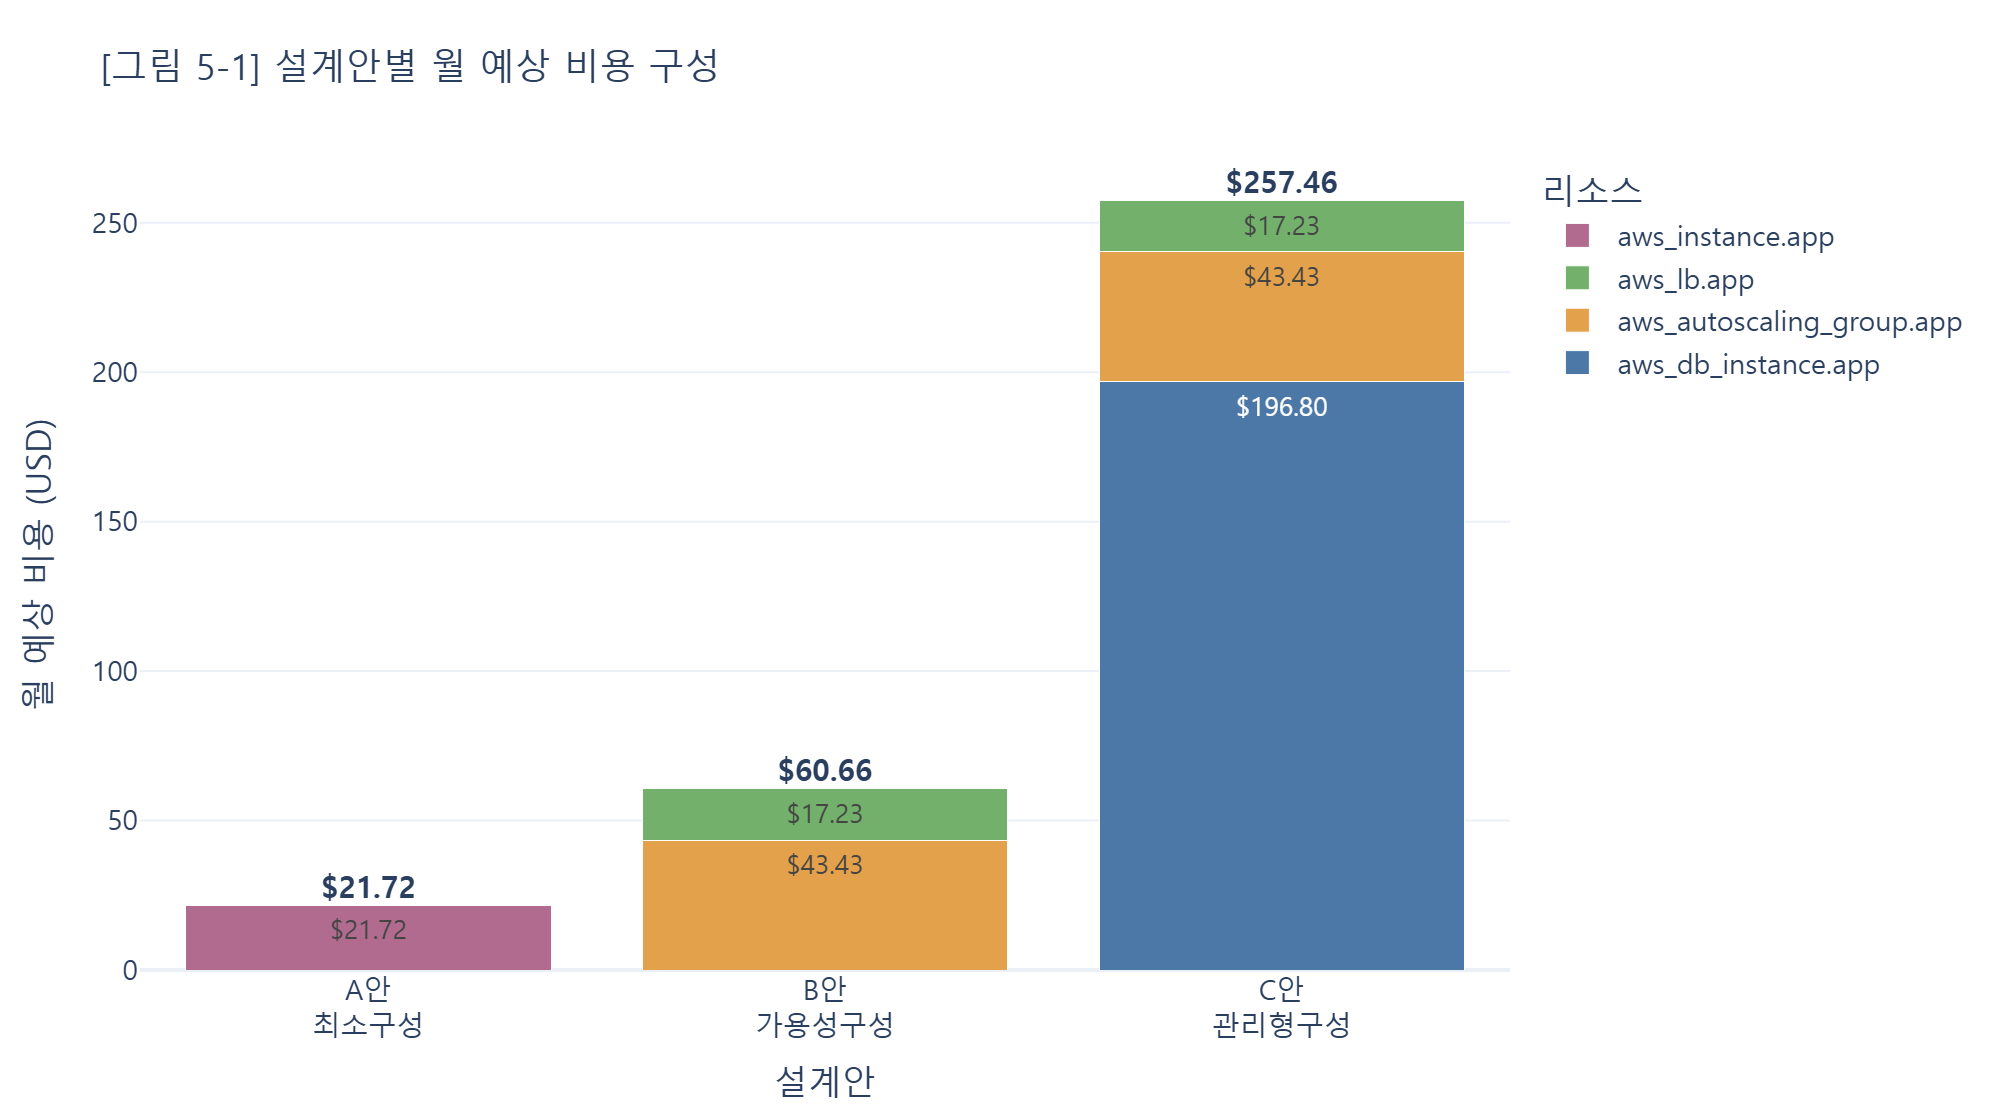
\includegraphics[width=\linewidth]{figure/fig_5_1_cost_breakdown.png}
\caption{설계안별 월 예상 비용 구성}
\label{fig:breakdown}
\end{figure}

\subsubsection{인스턴스 사양을 올렸을 때}

서론에서 밝힌 ``얼마가 깎일지 몰라 겁이 나서 가장 작은 사양만 골랐다''는 상황을 그대로 실험하였다.

\begin{table}[!h]
\centering
\caption{인스턴스 타입에 따른 비용 변화 (단위: USD)}
\label{tab:instancetype}
\small
\begin{tabularx}{\textwidth}{Y r r r r}
\toprule
\textbf{설계안} & \textbf{t3.small} & \textbf{t3.large} & \textbf{증가액} & \textbf{증가율} \\
\midrule
A안 & 21.72  & 78.66  & +56.94  & +262.2\% \\
B안 & 60.66  & 174.54 & +113.88 & +187.7\% \\
C안 & 257.46 & 371.34 & +113.88 & +44.2\% \\
\bottomrule
\end{tabularx}
\end{table}

\begin{figure}[!h]
\centering
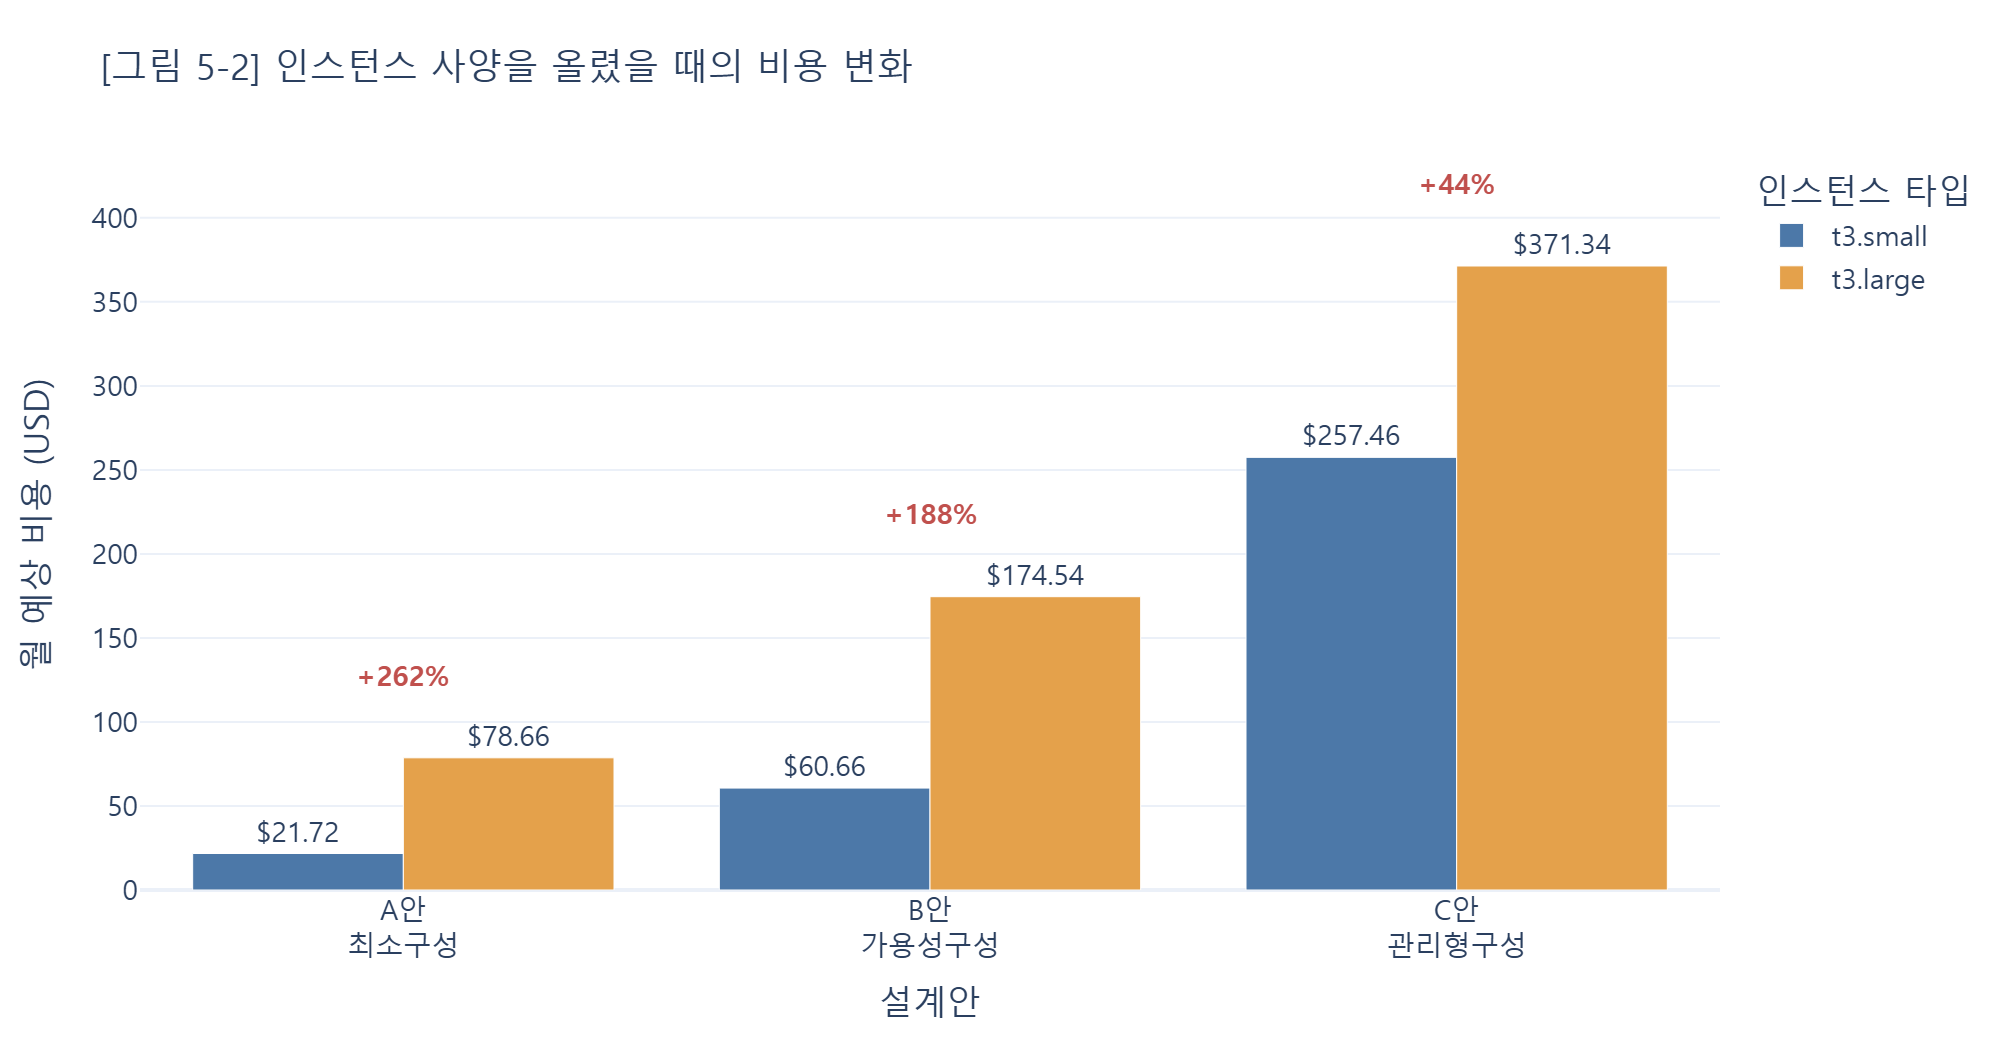
\includegraphics[width=\linewidth]{figure/fig_5_2_instance_type.png}
\caption{인스턴스 사양을 올렸을 때의 비용 변화}
\label{fig:instancefig}
\end{figure}

\subsubsection{DB 엔진 버전을 바꿨을 때}

C안의 비용 1위 리소스를 들여다보다가 예상하지 못한 항목을 발견하였다. RDS 비용 196.80달러 가운데 \textbf{175.20달러가 확장 지원(Extended Support) 요금}이었다. 표준 지원이 끝난 엔진 버전을 사용하면 AWS가 별도로 부과하는 요금이다.

\begin{table}[!h]
\centering
\caption{DB 엔진 버전에 따른 비용 변화 (단위: USD)}
\label{tab:engineversion}
\small
\begin{tabularx}{\textwidth}{Y r r r}
\toprule
\textbf{항목} & \textbf{MySQL 8.0} & \textbf{MySQL 9.0} & \textbf{차이} \\
\midrule
DB 인스턴스 (db.t3.micro, 730시간) & 18.98 & 18.98 & --- \\
스토리지 (gp3 20GB) & 2.62 & 2.62 & --- \\
확장 지원 (year 1) & 175.20 & 없음 & $-$175.20 \\
\midrule
\textbf{RDS 소계} & \textbf{196.80} & \textbf{21.60} & \textbf{$-$175.20} \\
\textbf{C안 총액} & \textbf{257.46} & \textbf{82.26}  & \textbf{$-$175.20} \\
\bottomrule
\end{tabularx}
\end{table}

\begin{figure}[!h]
\centering
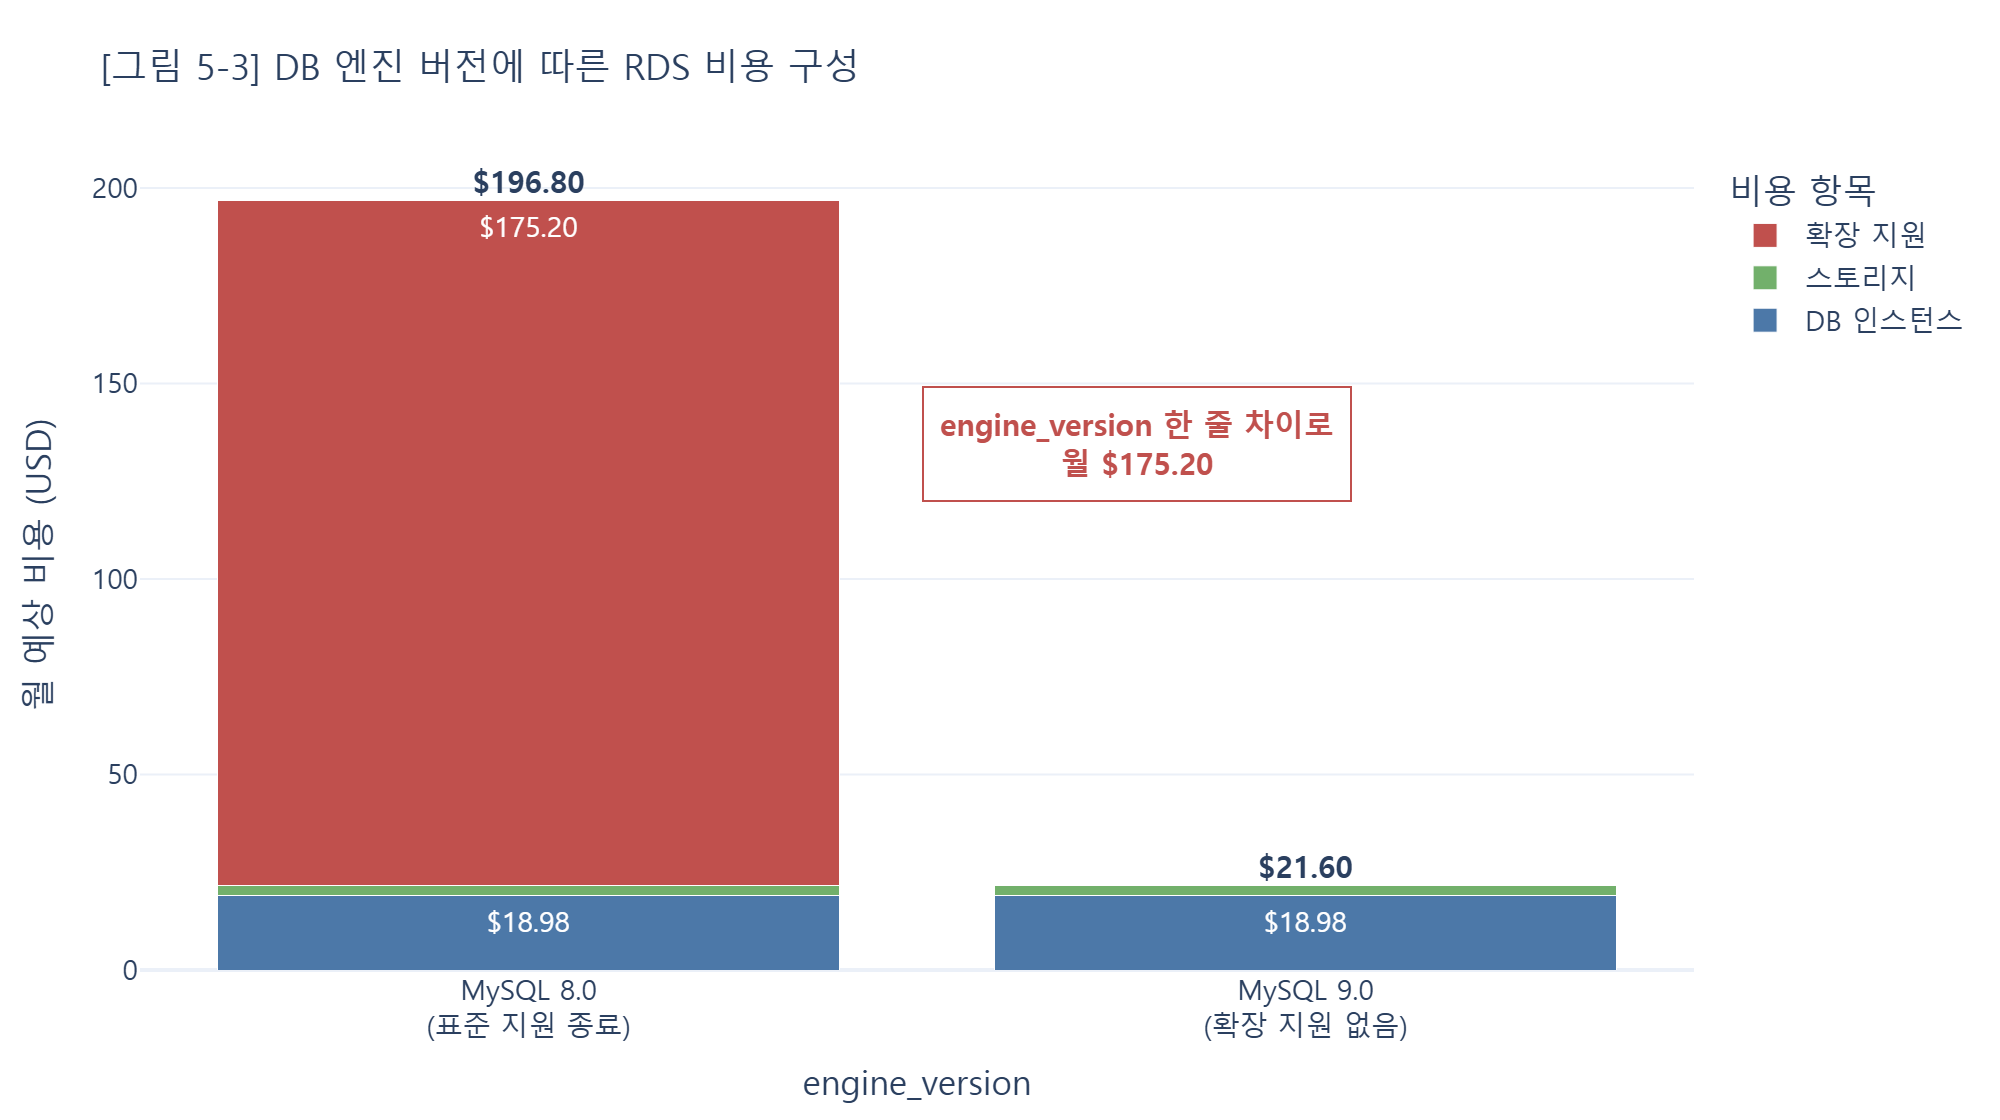
\includegraphics[width=\linewidth]{figure/fig_5_3_engine_version.png}
\caption{DB 엔진 버전에 따른 RDS 비용 구성}
\label{fig:enginefig}
\end{figure}

코드에서 달라지는 것은 \code{engine_version} 문자열 한 줄뿐이다. 그런데 월 비용은 175.20달러, DB 인스턴스 자체 요금(18.98달러)의 \textbf{9.2배}가 차이 난다.

\subsubsection{해석}

\paragraph{(1) 가용성의 가격은 서버 한 대 값이 아니다}
A안에서 B안으로 가면 월 38.94달러가 는다. 직관적으로는 ``서버가 1대에서 2대가 되니 두 배''일 것 같지만, 실제로는 \textbf{2.79배}가 된다. 늘어난 금액 가운데 인스턴스 추가분은 18.98달러뿐이고, 나머지 17.23달러는 로드 밸런서 요금이다. 즉 \textbf{가용성의 비용은 서버 대수가 아니라 트래픽을 나누는 장치에서 더 크게 발생한다.} 설계안을 머릿속으로만 비교해서는 알기 어려운 부분이다.

\paragraph{(2) 관리형 DB가 비싼 것이 아니라, 엔진 버전이 비쌌다}
C안은 A안의 11.9배로, 표면적으로는 ``관리형 DB는 감당 못 할 만큼 비싸다''는 결론으로 이어지기 쉽다. 그러나 5.3.3에서 확인했듯 B안 대비 증가분 196.80달러 가운데 \textbf{89\%인 175.20달러가 엔진 버전 때문}이고, 관리형 DB 자체의 값은 21.60달러에 지나지 않는다. 엔진 버전을 바꾸면 C안은 82.26달러로, B안 대비 35.6\% 증가에 그친다.

만약 이 도구 없이 설계했다면 ``RDS는 너무 비싸니 쓰지 말자''는 잘못된 결론에 도달했을 것이다. \textbf{문제는 선택지가 비싼 것이 아니라, 무엇이 비싼지를 몰랐다는 데 있었다.} 서론에서 ``문제는 비싸다는 것이 아니라 모른다는 것''이라고 규정한 바가 측정 결과로 확인된 셈이다.

\paragraph{(3) 같은 사양 변경이라도 체감이 다르다}
표~\ref{tab:instancetype}에서 t3.small을 t3.large로 올렸을 때, 증가액은 B안과 C안이 113.88달러로 같지만 증가율은 187.7\%와 44.2\%로 크게 다르다. 이미 다른 데서 큰 비용이 나가고 있으면 같은 변경이 작아 보인다. \textbf{학생이 ``이 정도는 괜찮겠지''를 판단할 때 기준이 되는 것은 절대 금액이 아니라 전체 구성 안에서의 비중}이며, 그래서 Cost Compass는 총액과 함께 리소스별 기여도를 항상 같이 보여 준다(4.3의 전체와 부분 분리).

\paragraph{(4) 이 도구가 필요한 이유를 스스로 증명하였다}
확장 지원 요금은 필자가 템플릿을 작성할 때 전혀 의도하지 않은 항목이었다. 평소 하던 대로 \code{engine_version = "8.0"}이라고 적었을 뿐인데 월 175달러가 붙었고, 그 사실을 \textbf{배포하기 전에, 크레딧을 한 푼도 쓰지 않고} 알게 되었다. 이 프로젝트가 가정한 사용자, 즉 아무것도 모르고 겁먹는 학생이 바로 필자 자신이었으며, 도구가 의도한 대로 작동한 사례가 되었다.

\subsection{한계점과 어려웠던 점}

\paragraph{(1) 도구 버전에 따른 가격 데이터 오차}
확장 지원 요금이 부과되는 기준을 확인하기 위해 엔진 버전을 바꿔 가며 측정한 결과는 다음과 같았다.

\begin{table}[!h]
\centering
\caption{엔진 버전별 확장 지원 부과 여부 (Infracost v0.10.47)}
\label{tab:enginethreshold}
\small
\begin{tabularx}{\textwidth}{Y l r}
\toprule
\textbf{engine\_version} & \textbf{확장 지원} & \textbf{C안 총액} \\
\midrule
8.0   & 부과 & 257.46 \\
8.4   & 부과 & 257.46 \\
8.4.3 & 부과 & 257.46 \\
9.0   & 없음 & 82.26 \\
\bottomrule
\end{tabularx}
\end{table}

즉 이 버전은 \textbf{9.0 미만을 일괄적으로 확장 지원 대상으로 취급}한다. 그러나 MySQL 8.4는 LTS 릴리스로 표준 지원 기간이 남아 있어, 실제 AWS 청구에서는 확장 지원 요금이 붙지 않을 가능성이 높다. 도구의 가격 데이터가 최신 상태를 반영하지 못한 것으로 보인다.

이 경험은 강의자료에서 제시한 오픈소스 선정 기준 가운데 \textbf{관리, 즉 최근까지 업데이트가 이어지는가} 항목이 왜 중요한지를 보여 준다. 저장소 자체는 활발히 관리되고 있었음에도(최신 릴리스가 측정 2주 전 공개), 특정 영역의 데이터는 뒤처져 있었다. 따라서 \textbf{표~\ref{tab:engineversion}의 차이 자체는 신뢰할 수 있으나, 어느 버전이 실제 과금 대상인지는 AWS 공식 문서로 교차 확인해야 한다.}

\paragraph{(2) 버전 체계의 불일치}
CLI는 실행할 때마다 v2.18.3으로 업데이트하라고 안내하였으나, 오픈소스 저장소의 릴리스 목록에는 해당 버전이 없고 v0.10.47이 최신이었다. 2.x 계열이 어떤 경로로 배포되는지는 확인하지 못했다. 이는 2.6에서 지적한 ``라이선스가 허용하는 자유와 실제로 독립적으로 운용할 수 있는 범위가 일치하지 않는다''는 문제와 맞닿아 있다.

\paragraph{(3) 가정값에 대한 민감도}
사용량 기반 항목은 가정값에 따라 결과가 달라진다. 본 비교는 세 설계안에 같은 가정을 적용하여 \textbf{상대적 순서}를 비교한 것이며, 절대 금액의 정확도를 보장하지 않는다. 특히 t3 계열은 버스터블 인스턴스여서 CPU 크레딧 초과 사용분이 추가로 과금되는데, 본 측정에서는 이를 0으로 가정하였다.

\paragraph{(4) 일부 리소스가 비용에 반영되지 않음}
A안에 포함한 \code{aws_eip}가 결과에 비용 0으로 처리되어, A안의 비용 1위 리소스 비중이 100\%로 나타났다. AWS는 2024년 2월부터 사용 중인 공인 IPv4 주소에도 요금을 부과하므로 실제로는 비용이 발생할 수 있다. 이 역시 (1)과 같은 성격의 데이터 한계로 보이나 확정하지 못하였다.

\paragraph{(5) 트래픽 비용이 A안에만 반영되지 않아 고트래픽 비교가 왜곡됨}
사용량 파일에 로드 밸런서의 처리 데이터량만 지정하고, EC2 인스턴스의 아웃바운드 데이터 전송량은 지정하지 않았다. 그 결과 \textbf{로드 밸런서가 없는 A안은 트래픽이 늘어도 비용이 전혀 변하지 않는다.}

\begin{table}[!h]
\centering
\caption{트래픽에 따른 설계안별 비용 변화 (단위: USD)}
\label{tab:traffic}
\small
\begin{tabularx}{\textwidth}{Y r r r}
\toprule
\textbf{월 데이터 전송량} & \textbf{A안} & \textbf{B안} & \textbf{C안} \\
\midrule
100 GB    & 21.72 & 60.66  & 257.46 \\
1,000 GB  & 21.72 & 67.86  & 264.66 \\
5,000 GB  & 21.72 & 99.86  & 296.66 \\
20,000 GB & 21.72 & 219.86 & 416.66 \\
\bottomrule
\end{tabularx}
\end{table}

실제 AWS는 EC2에서 인터넷으로 나가는 데이터 전송에도 요금을 부과하므로, A안의 고트래픽 구간 비용은 \textbf{과소 추정된 값}이다. 따라서 트래픽을 크게 높인 구간에서 A안과 다른 안을 직접 비교하는 것은 적절하지 않다. 본 보고서의 비교(100 GB 기준)는 이 왜곡이 작은 구간에서 이루어졌다.

덧붙여, 세 설계안의 비용 순서는 측정한 전 구간에서 A $<$ B $<$ C로 유지되었고 순위가 뒤바뀌는 지점은 나타나지 않았다. 4.2에서 후보로 낸 `손익분기점 찾기'는 이 세 가지 구성에서는 성립하지 않는 아이디어였던 셈이다. 4.4의 가중 순위 결정법에서 이 후보의 검증 가능성에 2점을 준 근거가 ``교차점이 실제로 존재할지 미리 보장할 수 없다''였는데, 그 우려가 그대로 확인되었다. 손익분기가 의미를 가지려면 고정비와 변동비의 구성이 서로 다른 설계안(예: 서버리스와 상시 가동 인스턴스)을 함께 놓아야 한다.

\paragraph{(6) 할인 제도 미반영}
Savings Plans, Reserved Instance, 프리 티어 등 실제 청구에 큰 영향을 주는 할인 제도는 반영되지 않았다. 학생이 받는 교육용 크레딧의 적용 방식 또한 반영되지 않으므로, 실제 차감액은 추정치와 다를 수 있다.

\paragraph{(7) 설계안 3종의 대표성}
미리 준비한 템플릿 바깥의 구성은 비교할 수 없다. 이는 시간 분리를 적용하면서 치른 대가이다. 구체화를 미리 해 두었기 때문에 사용자가 편해진 대신, \textbf{미리 준비된 선택지 안에서만} 비교가 가능해졌다.

\paragraph{(8) 작업 과정에서 겪은 문제}

\begin{table}[!h]
\centering
\caption{작업 과정에서 겪은 문제와 해결}
\label{tab:troubles}
\footnotesize
\begin{tabularx}{\textwidth}{Y Y}
\toprule
\textbf{문제} & \textbf{원인과 해결} \\
\midrule
\code{--config-file}과 \code{--terraform-var}를 함께 쓰면 실행되지 않음 & 도움말에 ``Cannot be used with path, terraform* or usage-file flags''로 명시되어 있었다. 변수를 명령행 대신 설정 파일의 \code{terraform_vars} 항목으로 넘겨 해결하였다. \\
사용량 파일의 키 이름이 실제와 달랐음 & 손으로 작성한 초안의 키가 맞지 않았다. \code{--sync-usage-file} 옵션으로 리소스에 맞는 키를 자동 생성한 뒤 값만 수정하였다. \\
\code{--sync-usage-file} 실행 시 \code{AuthFailure} 경고 & 사용량을 실제 AWS에서 조회해 추정하려다 자격 증명이 없어 실패한 것이다. 비용 계산에는 영향이 없었으며, 오히려 이 도구가 클라우드 자격 증명 없이 동작한다는 점(2.2.2)을 확인해 주는 결과였다. \\
리소스 비용 합계가 총액의 두 배 가까이 나옴 & 부모 리소스의 비용이 하위 리소스를 포함하는데 둘 다 더하고 있었다. 5.2 (3)의 방식으로 해결하고, 합계가 어긋나면 경고하도록 하였다. \\
한글 Windows 콘솔에서 스크립트가 중단됨 & cp949 인코딩이 일부 문자를 처리하지 못해 \code{UnicodeEncodeError}가 발생하였다. 표준 출력을 UTF-8로 재설정하여 해결하였다. \\
화면에서 설정을 바꿔도 이전 결과가 표시됨 & 캐시가 결과 파일 경로만 돌려주는데 모든 설정이 같은 파일을 쓰고 있었다. 설정 조합의 해시를 파일 이름에 넣어 분리하였다. \\
\bottomrule
\end{tabularx}
\end{table}

% =====================================================================
\section{결론 및 향후 계획}

\subsection{결과 요약}

본 보고서는 교육용 크레딧으로 실습하는 학생이 비용을 몰라 겁을 내고, 그 결과 가장 작은 사양만 고르게 되어 배울 기회를 잃는다는 문제에서 출발하였다.

5 Whys로 원인을 추적한 결과 ``비용을 알려면 설계를 확정해야 하고, 설계를 확정하려면 비용을 알아야 한다''는 순환 구조가 드러났고, 이를 \textbf{설계안의 구체성}을 특성으로 하는 물리적 모순으로 정의하였다. TRIZ의 시간 분리와 공간 분리를 적용하여, 구체화 작업을 비교 시점보다 앞으로 옮김으로써 \textbf{계산기에게는 완전히 구체적이면서 사용자에게는 아직 확정되지 않은 설계안}이라는 상태를 동시에 만들 수 있었다.

이를 구현하기 위해 다섯 개의 오픈소스를 하나의 파이프라인으로 연결하였다. OpenTofu로 설계안을 코드화하고, Infracost로 비용을 환산하며, pandas로 비교표를 만들고, Plotly와 Streamlit으로 학생이 직접 조작할 수 있는 화면을 제공하였다.

그 가운데 \textbf{Infracost의 역할이 가장 크게 바뀌었다.} 원래 이 도구는 실무 엔지니어가 이미 작성한 코드의 비용 변화를 \textbf{통제}하기 위한 것이다. 본 프로젝트는 이를 학생이 아직 정하지 않은 설계를 \textbf{선택}하기 위한 것으로 바꾸었다. 비용이 설계 이후에 통보받는 결과가 아니라, 설계를 고르는 기준의 하나가 된 것이다.

실제 측정 과정에서 이 전환의 효용이 예상하지 못한 방식으로 확인되었다. C안의 데이터베이스 비용 가운데 89\%가 관리형 서비스 자체가 아니라 \textbf{표준 지원이 끝난 엔진 버전에 부과되는 확장 지원 요금}이었다(5.3.3). 코드에서는 버전 문자열 한 줄로만 보이지만 월 175달러였고, 이를 모른 채 설계했다면 ``관리형 데이터베이스는 너무 비싸다''는 잘못된 결론에 이르렀을 것이다. 필자 자신이 이 프로젝트가 가정한 사용자였던 셈이며, 도구가 의도한 대로 작동한 사례가 되었다.

이 전환은 학생에게 특히 의미가 있다. 서론에서 밝혔듯 학생이 비용을 몰라서 잃는 것은 돈이 아니라 배울 기회였다. 설계안별 금액을 미리 확인할 수 있게 되면 학생은 \textbf{겁이 아니라 근거로} 선택하게 된다. 본 프로젝트가 궁극적으로 줄이려 한 것은 비용이 아니라, 비용을 몰라서 생기는 \textbf{불안}이다.

\subsection{혼자에서 함께로: 만든 것을 돌려놓기}

1.1에서 메이커가 된다는 것을 세 가지 변화로 정리하였다. 소비자에서 생산자로는 1.2에서 3장까지, 아이디어에서 프로토타입으로는 4장과 5장에서 다루었다. 남은 것이 \textbf{혼자에서 함께로}이다.

메이커 운동의 핵심은 \textbf{모든 것을 디지털화}하여 설계도, 코드, 데이터를 파일로 만들고, \textbf{기술과 지식을 나누어} 만드는 방법을 공개하고 함께 발전시키는 데 있다. 이를 한 줄로 요약한 것이 \textbf{DIY(Do It Yourself, 혼자 만든다)에서 DIT(Do It Together, 함께 만들고 나눈다)로}의 전환이다.

이 기준에서 보면, 다섯 개의 오픈소스를 받아 쓰기만 하고 끝내는 것은 절반만 한 일이다. 가져다 쓴 쪽에 머물면 생산자가 되었다고 보기 어렵다. 그래서 본 프로젝트의 결과물 전체를 공개 저장소에 올려 돌려놓았다~\cite{costcompass}.

\begin{table}[!h]
\centering
\caption{공개한 내용}
\label{tab:published}
\small
\begin{tabularx}{\textwidth}{l Y Y}
\toprule
\textbf{구분} & \textbf{내용} & \textbf{공개한 이유} \\
\midrule
설계안 코드 & \code{design-a/b/c}의 HCL 템플릿 & 같은 비교를 하려는 사람이 처음부터 작성하지 않아도 되게 \\
설정 파일 & 공통 사용량 가정, 사양과 엔진 버전 실험 설정 & 어떤 가정 위에서 나온 숫자인지 드러내기 위해 \\
분석 스크립트 & \code{analyze.py}, \code{make_figures.py}, \code{app.py} & 결과를 다시 만들어 볼 수 있도록 \\
\textbf{측정 결과 원본} & \code{result*.json} & \textbf{숫자를 주장만 하지 않고 검증할 수 있게 하기 위해} \\
보고서 & 본 문서와 조판 소스 & 결론만이 아니라 도달한 과정을 함께 남기기 위해 \\
\bottomrule
\end{tabularx}
\end{table}

특히 측정 결과 JSON을 포함한 것은 의도한 선택이다. 강의자료는 오픈소스를 쓸 때 ``결과는 정직하게, 잘 된 점과 한계를 구분해 쓴다''고 요구한다. 보고서에 적은 숫자가 맞는지 독자가 직접 확인할 수 있어야 그 요구를 충족한다고 보았다. 5.4에 정리한 한계도 숨기지 않고 저장소 문서에 그대로 적었다.

공개의 의미가 가장 분명해지는 지점은 5.3.3의 확장 지원 요금이다. 필자는 \code{engine_version} 한 줄 때문에 월 175달러가 붙는다는 사실을 모른 채 템플릿을 작성했고, 도구를 돌려 보고서야 알게 되었다. 이 경험을 혼자 알고 끝내면 다음 사람이 똑같이 당한다. 코드와 측정 결과를 함께 공개해 두면 \textbf{한 사람이 치른 시행착오가 다음 사람에게는 이미 해결된 출발점}이 된다. 이것이 DIY와 DIT의 차이이며, 메이커 운동이 말하는 ``함께 만들며 발전시킴''의 가장 작은 단위라고 생각한다.

덧붙여, 본 프로젝트는 3D 프린터나 별도의 장비 없이 \textbf{노트북 한 대로} 수행되었다. 강의자료가 ``소프트웨어 메이커는 노트북 한 대면 충분하다''고 한 것을 그대로 확인한 셈이다.

결국 1.1에서 던진 물음으로 돌아온다. 만드는 일은 오픈소스가 대부분 해결해 주었고, 장비도 필요하지 않았다. 끝까지 남았던 어려움은 \textbf{무엇을 만들지 정하는 일}이었다. 그 답을 찾기 위해 한 일은 새로운 기술을 배우는 것이 아니라, 내가 겪은 불편을 다시 들여다보고 그것을 다른 사람도 겪는 문제로 정의하는 것이었다. 이번 과제에서 얻은 것은 비용 비교 도구 하나가 아니라, 만들 것을 찾는 방법이었다고 생각한다.

\subsection{향후 계획}

첫째, 설계안 템플릿을 늘려 대표성 한계를 완화한다. 둘째, 비용과 가용성을 함께 놓고 보는 2축 비교(4.2의 후보 6)를 도입하여, 비용만으로 설계를 판단하게 되는 부작용을 막는다. 셋째, 4.4에서 기간 문제로 보류한 \textbf{후보 3(예산 역산)}을 다시 다룬다. 교육용 크레딧의 잔액을 입력하면 ``이 구성으로 며칠을 버틸 수 있는가''를 환산해 주는 형태가 출발점이 될 수 있다. 학생이 실제로 쥐고 있는 단위는 월 달러가 아니라 남은 크레딧이기 때문이다.

저장소는 공개 상태로 유지하여, 위 계획이 진행되는 과정도 함께 기록할 것이다.

% =====================================================================
\newpage
{
\small
\bibliographystyle{unsrt}
\bibliography{refer}
}

\end{document}
